%%%%%%%%%%%%%%%%%%%%%%%%%%%%%%%%%%%%%%%%%%%%%%%%%%%%%%%%%%%%%%%%%%%%%%
%  Run mode: pdfLaTeX
%  !Mode: "Tex:Utf-8"
%  Authors: Xiangdong Jia
%  Date: Last Updated May-30-2023
%  Copyright UWC&IoT@NWNU
%%%%%%%%%%%%%%%%%%%%%%%%%%%%%%%%%%%%%%%%%%%%%%%%%%%%%%%%%%%%%%%%%%%%%%
\def\usewhat{dvipdfmx}                              % 定义编译方式 dvipdfmx 或者 pdflatex,默认为 dvipdfmx
                                                    % 方式编译,如果需要修改,只需改变花括号中的内容即可。
%\setlength{\baselineskip}{20pt}
%\setlength{\headheight}{25pt}

\documentclass[a4paper,12pt,openany,twoside]{book}

                                           % 如果论文超过 60 页 可以使用 twoside 双面打印
% !Mode:: "TeX:UTF-8"
%西北师范大学 贾向东教授 无线通信实验室

%%%%%%%%%% Package %%%%%%%%%%%%
%\usepackage{fontspec}
%\usepackage{xunicode}
%\usepackage{xltxtra}
\usepackage{times}
\usepackage{enumerate}
\usepackage[chapter]{algorithm}
\usepackage{algorithmic}
\usepackage{graphicx}                       % 支持插图处理
\usepackage{geometry}
%\usepackage{geometry}
\geometry{left=3.0cm,right=3.0cm,top=3.0cm,bottom=3.0cm}%%%%%%%页面边距的设置
%\geometry{left=2.5cm,right=2.5cm,top=2cm,bottom=2.5cm,footskip=1.1cm,headsep=0.7cm,head=0.4cm}
                                            % 支持版面尺寸设置
\usepackage{titlesec}                       % 控制标题的宏包
\usepackage{titletoc}                       % 控制目录的宏包
\usepackage{fancyhdr}                       % fancyhdr 宏包 支持页眉和页脚的相关定义
\usepackage[UTF8]{ctex}                     % 支持中文显示
\usepackage{cite}
\usepackage{color}                          % 支持彩色
\usepackage{amsmath}                        % AMSLaTeX 宏包 用来排出更加漂亮的公式
\usepackage{amssymb}                        % 数学符号生成命令
\usepackage[below]{placeins}                %允许上一个 section 的浮动图形出现在下一个 section 的开始部分,还提供\FloatBarrier 命令,使所有未处理的浮动图形立即被处理
\usepackage{flafter}                        % 使得所有浮动体不能被放置在其浮动环境之前,以免浮动体在引述它的文本之前出现。
\usepackage{multirow}                       % 使用 Multirow 宏包,使得表格可以合并多个 row 格
\usepackage{booktabs}                       % 表格,横的粗线;\specialrule{1pt}{0pt}{0pt}
\usepackage{longtable}                      % 支持跨页的表格。
\usepackage{tabularx}                       % 自动设置表格的列宽
\usepackage{setspace}
\usepackage{subfigure}                      % 支持子图 %centerlast 设置最后一行是否居中
\usepackage[subfigure]{ccaption}            % 支持子图的中文标题
\usepackage[sort&compress,numbers]{natbib}  % 支持引用缩写的宏包
\usepackage{enumitem}                       % 使用 enumitem 宏包,改变列表项的格式
\usepackage{enumerate}
\usepackage{calc}                           % 长度可以用 + - * / 进行计算
\usepackage{txfonts}                        % 字体宏包
\usepackage{bm}                             % 处理数学公式中的黑斜体的宏包
\usepackage[amsmath,thmmarks,hyperref]{ntheorem}  % 定理类环境宏包,其中 amsmath 选项用来兼容 AMS LaTeX 的宏包
\usepackage{CJKnumb}                        % 提供将阿拉伯数字转换成中文数字的命令
\usepackage{indentfirst}                    % 首行缩进宏包
\usepackage{CJKutf8}                        % 用在 UTF8 编码环境下,它可以自动调用 CJK,同时针对 UTF8 编码作了设置。
\usepackage{CJK}
\usepackage{fancyhdr}
\usepackage{lastpage}
\usepackage{layout}
\usepackage[titles,subfigure]{tocloft}
                     %控制生成的表格和图片的目录格式
\usepackage{caption}

\usepackage{ragged2e}
% \usepackage{expl3}

%\usepackage{hypbmsec}                      % 用来控制书签中标题显示内容

%如果您的 pdf 制作中文书签有乱码使用如下命令,就可以解决了
\usepackage[pdftex, unicode,               % pdflatex, pdftex 这里决定运行文件的方式不同
            pdfstartview=FitH,
            %CJKbookmarks=true,
            bookmarksnumbered=true,
            bookmarksopen=true,
            colorlinks=true,
            pdfborder={0 0 1},
            citecolor=black,
            linkcolor=black,
            anchorcolor=black,
            urlcolor=black,
            breaklinks=true
            ]{hyperref}

% \usepackage{setup/bibspacing}
\renewcommand{\theequation}{\arabic{chapter}-\arabic{equation}}
\makeatletter
\def\tagform@#1{\maketag@@@{(\ignorespaces#1\unskip)}}
\makeatother

                      % 定义本文所使用宏包
\graphicspath{{figures/}}
\usepackage{amsmath}                       % 开始中文字体使用
\usepackage{url}
\usepackage{CJK}
%\usepackage{tabu}
\usepackage{enumerate}
\DeclareCaptionFont{myfont}{\fontsize{10.5pt}{10.5pt}\selectfont}
\captionsetup[algorithm]{font=myfont}

                 % 定义所有的.eps 文件在 figures 子目录下
\begin{document}
\begin{sloppypar}                          % 开始全文
\begin{CJK*}{UTF8}{song}


\pagestyle{empty}
%%%%%%%%%%%%%%%%%%%%%%%%%%%%%%%%%%%%%%%%%%%%%%%%%%%%%%%%%%%%%%%%%%%%%%
%  run mode: pdfLatex on WinEdt10.3
%  !Mode: "Tex:Utf-8"
%  Authors: Xiangdong Jia and Mangang Xie from UWC&IoT Lab
%  Copyright: 泛在无线通信与物联网实验室@计算机科学与工程学院@西北师范大学
%  Version: 2023 年 6 月 1 日
%%%%%%%%%%%%%%%%%%%%%%%%%%%%%%%%%%%%%%%%%%%%%%%%%%%%%%%%%%%%%%%%%%%%%%


%%%%%%%%%% Fonts Definition and Basics %%%%%%%%%%%%%%%%%
\renewcommand{\today}{二〇二三年五月}     %封面第一页的日期定义
\newcommand{\song}{\CJKfamily{song}}    % 宋体
%\newcommand{\FSGB}{\CJKfamily{FSGB}}
%\setCJKfamilyfont{FSGB}{仿宋_GB2312.ttf}
\newcommand{\FSGB}{\CJKfamily{FSGB}} %仿宋 GB2312
\newcommand{\fs}{\CJKfamily{fs}}        % 仿宋体
\newcommand{\kai}{\CJKfamily{kai}}      % 楷体
\newcommand{\hei}{\CJKfamily{hei}}      % 黑体
\newcommand{\li}{\CJKfamily{li}}        % 隶书
\newcommand{\yihao}{\fontsize{26pt}{26pt}\selectfont}       % 一号,1.倍行距
\newcommand{\xiaoyi}{\fontsize{24pt}{24pt}\selectfont}      % 小一,1.倍行距
\newcommand{\erhao}{\fontsize{22pt}{22pt}\selectfont}       % 二号,1.倍行距
\newcommand{\er}{\fontsize{20pt}{20pt}\selectfont}       % 20pt, 单倍行距
\newcommand{\xiaoer}{\fontsize{18pt}{18pt}\selectfont}      % 小二,单倍行距
\newcommand{\sanhao}{\fontsize{16pt}{16pt}\selectfont}      % 三号,1.倍行距
\newcommand{\xiaosan}{\fontsize{15pt}{15pt}\selectfont}     % 小三,1.倍行距
\newcommand{\sihao}{\fontsize{14pt}{14pt}\selectfont}       % 四号,1.0 倍行距
%\newcommand{\xiaosi}{\fontsize{12.5pt}{12.5pt}\selectfont}      % 小四,1.倍行距
\newcommand{\xiaosi}{\fontsize{12pt}{12pt}\selectfont}      % 小四,1.倍行距
\newcommand{\wuhao}{\fontsize{10.5pt}{10.5pt}\selectfont}   % 五号,单倍行距
\newcommand{\xiaowu}{\fontsize{9pt}{9pt}\selectfont}        % 小五,单倍行距

\setlength{\headheight}{24pt}%%%%%%%%%%%%页眉和上边距之间的距离%%%%%%%%%%%%%%%%%%%%%%%%%%%%%
%\setlength{\headsep}{20pt}
%\setlength{\footskip}{4pt}
\setlength{\textheight}{23cm}%%%%%%%%%%%%%%%%%%%%%%%%%%%%%%%%%%设置内容高度
%\newcommand{\abstractname}{摘要}
%\CJKcaption{gb_452}
\CJKtilde  % 重新定义了波浪符~的意义

\newcommand\prechaptername{第}
\newcommand\postchaptername{章}

% 调整罗列环境的布局
\setitemize{leftmargin=3em,itemsep=0em,partopsep=0em,parsep=0em,topsep=-0em}
\setenumerate{leftmargin=3em,itemsep=0em,partopsep=0em,parsep=0em,topsep=0em}


%避免宏包 hyperref 和 arydshln 不兼容带来的目录链接失效的问题。
\def\temp{\relax}
\let\temp\addcontentsline
\gdef\addcontentsline{\phantomsection\temp}

% 自定义项目列表标签及格式 \begin{publist} 列表项 \end{publist}
\newcounter{pubctr} %自定义新计数器
\newenvironment{publist}{%%%%%定义新环境
\begin{list}{[\arabic{pubctr}]} %%标签格式
    {
     \usecounter{pubctr}
     \setlength{\leftmargin}{4em}     % 左边界 \leftmargin =\itemindent + \labelwidth + \labelsep
     \setlength{\itemindent}{0em}     % 标号缩进量
     \setlength{\labelsep}{1em}       % 标号和列表项之间的距离,默认 0.5em
     \setlength{\rightmargin}{0em}    % 右边界
     \setlength{\topsep}{0ex}         % 列表到上下文的垂直距离
     \setlength{\parsep}{0ex}         % 段落间距
     \setlength{\itemsep}{0ex}        % 标签间距
     \setlength{\listparindent}{0pt} % 段落缩进量
    }}
{\end{list}}%%%%%

%%%%%%%%%%%%%%%%%%%%%%%%%%%%%%%%%%%%%%%%%%%%%%%%%%5默认字体大小
\makeatletter
\renewcommand\normalsize{
  \@setfontsize\normalsize{12pt}{12pt} % 小四对应 12pt
  \setlength\abovedisplayskip{4pt}
  \setlength\abovedisplayshortskip{4pt}
  \setlength\belowdisplayskip{\abovedisplayskip}
  \setlength\belowdisplayshortskip{\abovedisplayshortskip}
    \let\@listi\@listI}
%%%%%%%%%%%%%%%%%%%%%%%%-5555555555555                                 -------定义默认字体和行距---------%%%%%%%%%%%%%%%%%%%%%%%%%%%%%%%%%%%%%%%%%%%%%
%\renewcommand{\CJKglue}{\hskip 0.5pt \baselineskip}
\def\defaultfont{\renewcommand{\baselinestretch}{1.67}\normalsize\selectfont}

%\def\defaultfont{\renewcommand{\baselinestretch}{1.83}\normalsize\selectfont}
%\setlength{\baselineskip}{20pt}

% %%%%%%%%%%%%%%%%%%%%%%%%%%%%%%%%%%%%%%%%%%%%%%%%%%%%%%%%设置行距和段落间垂直距离

\setlength{\baselineskip}{18pt}
%\renewcommand{\CJKglue}{\hskip 0.5pt plus \baselineskip} %加大字间距,使每行 35 个字
%\renewcommand{\CJKglue}{\hskip 1cm \baselineskip} %加大字间距,使每行 35 个字
\renewcommand{\CJKglue}{\hskip 0.5pt plus \baselineskip} %加大字间距,使每行 35 个字
%\renewcommand{\CJKglue}{\hskip 2pt plus 0.08\baselineskip}
%\renewcommand{\CJKglue}{\hskip 1cm}

\makeatother

%%%%%%%%%%%%% Contents %%%%%%%%%%%%%%%%%
%\pagestyle{empty}
%\fancyhf{}
%\thispagestyle{empty}

\renewcommand{\contentsname}{目\quad 录}

%\thispagestyle{empty}
\setcounter{tocdepth}{2}%%%%%%%%设置目录层次 的深度
\titlecontents{chapter}[0em]{\xiaosi\hei}%
             {\prechaptername~~\thecontentslabel~~\postchaptername~~~}{} %
             {\titlerule*[5pt]{$\cdot$}\xiaosi\contentspage}
\titlecontents{section}[1em]{\xiaosi\song} %
            {\thecontentslabel\quad }{} %
            {\hspace{.25em}\titlerule*[5pt]{$\cdot$}\xiaosi\contentspage}
\titlecontents{subsection}[2em]{\xiaosi\song} %
            {\thecontentslabel\quad }{} %
            {\hspace{.25em}\titlerule*[5pt]{$\cdot$}\xiaosi\contentspage}
\renewcommand{\cftdotsep}{1.1}
\renewcommand{\listfigurename}{图片索引}
\setcounter{lofdepth}{1}
%\titlefigures{chapter}[1em]{\xiaosi\hei}%
%             {\prechaptername~~\thecontentslabel~~\postchaptername~~~}{} %
%            {\titlerule*[5pt]{$\cdot$}\xiaosi\contentspage}
\renewcommand{\listtablename}{表格索引}



%%%%%%%%%%%%%%%%%%%%%%%%%%%%%%%%%%%%%%%%%定义页眉和页脚%%%%%%%%%%%%%%%%%%%%%%%%%%%%%%%%%%%
\makeatletter

\def\@chapter[#1]#2{\ifnum \c@secnumdepth >\m@ne
                       \if@mainmatter
                         \refstepcounter{chapter}%
                         \typeout{\@chapapp\space\thechapter.}%
                         \addcontentsline{toc}{chapter}%
                                   {\protect\numberline{\thechapter}#1}%
                         \def\leftmark{第\thechapter 章\quad #2}
                       \else
                         \addcontentsline{toc}{chapter}{#1}%
                       \fi
                    \else
                      \addcontentsline{toc}{chapter}{#1}%
                    \fi
                    \chaptermark{#1}%
                    \if@twocolumn
                      \@topnewpage[\@makechapterhead{#2}]%
                    \else
                      \@makechapterhead{#2}%
                      \@afterheading
                    \fi}

\def\@schapter#1{\if@twocolumn
                   \@topnewpage[\@makeschapterhead{#1}]%
                 \else
                   \@makeschapterhead{#1}%
                   \def\leftmark{#1}
                   \@afterheading
                 \fi}
\makeatother
%%%%%%%%%%%%%%%%%%%%%%%%%%%%%%%%%%%%%%%%%%%%%%%%%%%%%%%%%%%%%%%%%%%%%%%%%%%%%%%%%%%%%%%%%%%%%%%%%%%

%%%%%%%%%% %%%%%%%%%%%%%%%%%-----定义章节和小节的地方---%%%%%%% %%%%%%%%%%%%%%%%%
\setcounter{secnumdepth}{4}
\setlength{\parindent}{2em}
\renewcommand{\chaptername}{\prechaptername\arabic{chapter}\postchaptername}
\titleformat{\chapter}{\centering\sanhao\hei}{\chaptername}{1em}{}%%%%%%%%%%%%{\centering}Large  定义章标题居左
\titlespacing{\chapter}{0pt}{-10pt}{18pt}
\titleformat{\section}{\sihao\hei}{\thesection}{1em}{}
\titlespacing{\section}{0pt}{20pt}{8pt}
\titleformat{\subsection}{\sihao\hei}{\thesubsection}{1em}{}
\titlespacing{\subsection}{0pt}{20pt}{8pt}
\titleformat{\subsubsection}{\xiaosi\hei}{\thesubsubsection}{0.5em}{}
\titlespacing{\subsubsection}{0pt}{6pt}{6pt}
%%%%%%%%%%%%%%%%%%%%%%%%%%%%%%%%%%%%%%%%%%%%%%%%%%%%%%%%%%%%%%%%%%%%%%%%%%%%%%%%%%%%%

%%%%%%%%%% %%%%%%%%%%%%%%%%%%%%%%%%%%%%%  图和表的编号 格式 %%%%%%%%%  %%%%%%%%%%%%%%%%%
\renewcommand{\tablename}{\bfseries 表} % 插表题头
\renewcommand{\figurename}{\bfseries 图} % 插图题头
%\renewcommand{\figurename}{{\bfseries 图~\arabic{chapter}-\arabic{figure}}} % 插图题头
%\renewcommand{\thefigure}{}

\renewcommand{\thefigure}{\arabic{chapter}-\arabic{figure}} % 使图编号为 7.1 的格式 %\protect{~}
\renewcommand{\thetable}{\arabic{chapter}-\arabic{table}}%使表编号为 7.1 的格式
\renewcommand{\theequation}{\arabic{chapter}-\arabic{equation}}%使公式编号为 7.1 的格式
\renewcommand{\thesubfigure}{(\alph{subfigure})}%使子图编号为 (a) 的格式
\renewcommand{\thesubtable}{(\alph{subtable})} %使子表编号为 (a) 的格式
\makeatletter
\renewcommand{\p@subfigure}{\thefigure~} %使子图引用为 7.1 a) 的格式,母图编号和子图编号之间用~ 加一个空格

%\captionsetup[figure]{labelformat=simple, labelsep=space, skip=88pt, labelfont={bf}}
\captionsetup[figure]{skip=8pt} % 很重要的一个语句

\makeatother


%% %%%%%%%%%%%%%%%%%%%%%%%%%%%%%%%%%定制浮动图形和表格标题样式%%%%%%%%%%%%%%%%%%
\makeatletter
\long\def\@makecaption#1#2{%
   \vskip\abovecaptionskip
   \sbox\@tempboxa{\centering\wuhao{#1~~#2} }%
   \ifdim \wd\@tempboxa >\hsize
     \centering\wuhao{#1~~#2} \par
   \else
     \global \@minipagefalse
     \hb@xt@\hsize{\hfil\box\@tempboxa\hfil}%
   \fi
   \vskip\belowcaptionskip}
\makeatother
\captiondelim{~~~~} %用来控制 longtable 表头分隔符

\newcommand{\figref}[1]{{图~\ref{#1}}}
\newcommand{\tabref}[1]{{表~\ref{#1}}}

%\newcommand{\figref}[1]{{图~\arabic{chapter}-\arabic{figure}\ref{#1}}}

%%%%%%%%%%%%%%%%%%%%%%%%%%%%%%%%%%%%%%%%%%%%%定理、定义、猜想%%%%%%%%%%%%%%%%%%%%%%%%%%%%%%%%%%%
\theorembodyfont{\song\rmfamily}
\theoremheaderfont{\hei\rmfamily}
\newtheorem{theorem}{\hei 定理~}[chapter]
\newtheorem{lemma}{\hei 引理~}[chapter]
\newtheorem{axiom}{\hei 公理~}[chapter]
\newtheorem{proposition}{命题~}[chapter]
\newtheorem{corollary}{推论~}[chapter]
\newtheorem{definition}{定义~}[chapter]
\newtheorem{conjecture}{猜想~}[chapter]
\newtheorem{example}{例~}[chapter]
\newtheorem{remark}{注~}[chapter]
\floatname{algorithm}{算法}%将英文的 algorithm 改为算法

\renewcommand{\algorithmicrequire}{\textbf{Input:}}
\renewcommand{\algorithmicensure}{\textbf{Output:}}
%\captionsetup[algorithm]{font=footnotesize}%将算法标题改为 10.5

\newcommand{\tabincell}[2]{\begin{tabular}{@{}#1@{}}#2\end{tabular}}%表格合并
\newenvironment{proof}{\noindent{\hei 证明:}}{\hfill $ \square $ \vskip 4mm}
\theoremsymbol{$\square$}


%%%%%%%%%%% JXD definition  %%%%%%%%%%%%%
%定义环境变量 TheoremJXD, 定理
\newcounter{Theo}[chapter]
% 每当使用\newcounter 命令定义一个新的计数器时,系统将会自动自动地定义一条新命令,
%\newcounter{\the 新计数器\arabic{新计数器}},此命令可用于显示该计数器当前值\the
\newenvironment{TheoremJXD}{\refstepcounter{Theo}\vspace{5pt}\indent \kaishu{\bfseries 定理\arabic{chapter}-\arabic{Theo}:}~}{\kaishu\vspace{-10pt}}
% 引用方式
\newcommand{\TheoremJXDref}[1]{{定理~\arabic{chapter}-\ref{#1}}}

%\newenvironment{myenv}{\noindent 文档前面的内容\par}{文档后面的内容}
%\renewcommand{\myenv}[2]{\arabic{chapter}-\arabic{myenv}:\kaishu}
%\renewcommand{\theTheo}{{{Theorem}~\arabic{Theo}}}

%定义环境变量 LemmaJXD, 引理
\newcounter{Lemm}[chapter]
% 每当使用\newcounter 命令定义一个新的计数器时,系统将会自动自动地定义一条新命令,
%\newcounter{\the 新计数器\arabic{新计数器}},此命令可用于显示该计数器当前值\the
\newenvironment{LemmaJXD}{\refstepcounter{Lemm}\vspace{5pt}\indent \kaishu{\bfseries 引理\arabic{chapter}-\arabic{Lemm}:}~}{\kaishu\vspace{-10pt}}
% 引用方式
\newcommand{\LemmaJXDref}[1]{{引理~\arabic{chapter}-\ref{#1}}}


%定义环境变量 CorollaryJXD, 推论
\newcounter{Corol}[chapter]
% 每当使用\newcounter 命令定义一个新的计数器时,系统将会自动自动地定义一条新命令,
%\newcounter{\the 新计数器\arabic{新计数器}},此命令可用于显示该计数器当前值\the
\newenvironment{CorollaryJXD}{\refstepcounter{Corol}\vspace{5pt}\indent \kaishu{\bfseries 推论\arabic{chapter}-\arabic{Corol}:}~}{\kaishu\vspace{-10pt}}
% 引用方式
\newcommand{\CorollaryJXDref}[1]{{推论~\arabic{chapter}-\ref{#1}}}


%定义环境变量 CorollaryJXD, 定义 Definition
\newcounter{Defi}[chapter]
% 每当使用\newcounter 命令定义一个新的计数器时,系统将会自动自动地定义一条新命令,
%\newcounter{\the 新计数器\arabic{新计数器}},此命令可用于显示该计数器当前值\the
\newenvironment{DefinitionJXD}{\refstepcounter{Defi}\vspace{5pt}\indent \kaishu{\bfseries 定义\arabic{chapter}-\arabic{Defi}:}~}{\kaishu\vspace{-10pt}}
% 引用方式
\newcommand{\DefinitionJXDref}[1]{{定义~\arabic{chapter}-\ref{#1}}}


%定义环境变量 PropositionJXD, 命题
\newcounter{Prop}[chapter]
% 每当使用\newcounter 命令定义一个新的计数器时,系统将会自动自动地定义一条新命令,
%\newcounter{\the 新计数器\arabic{新计数器}},此命令可用于显示该计数器当前值\the
\newenvironment{PropositionJXD}{\refstepcounter{Prop}\vspace{5pt}\indent \kaishu{\bfseries 命题\arabic{chapter}-\arabic{Prop}:}~}{\kaishu\vspace{-10pt}}
% 引用方式
\newcommand{\PropositionJXDref}[1]{{命题~\arabic{chapter}-\ref{#1}}}


%%%%%%%%%% Page: number, header and footer  页码%%%%%%%%%%%%%%%%%

%\frontmatter 或 \pagenumbering{roman}
%\mainmatter 或 \pagenumbering{arabic}
\makeatletter
\renewcommand\frontmatter{\clearpage
  \@mainmatterfalse
  \pagenumbering{Roman}} % 正文前罗马字体编号
\makeatother


%%%%%%%%%%%%%%%%%%%%%%%%%%%%%%%%定制附录 格式%%%%%%%%%%%%%%%%%


\newcounter{sectionAppen}
\renewcommand{\thesectionAppen}{{\arabic{sectionAppen}}}
\newcommand{\sectionAppenJXD}[1]{\par\noindent\refstepcounter{sectionAppen}{\sihao\textbf{%
			\thesectionAppen:~#1}}\par\setlength{\parindent}{2em}}

\newcounter{subsectionAppen}%{sectionApen}
\renewcommand{\thesubsectionAppen}{{\arabic{subsectionAppen}}}
\newcommand{\subsectionAppenJXD}[1]{\vspace{8pt}\par\noindent\refstepcounter{subsectionAppen}{\sihao\textbf{\thesectionAppen.
			\thesubsectionAppen:~#1}}\par\setlength{\parindent}{2em}}
\makeatletter
\@addtoreset{subsectionAppen}{sectionAppen}
\makeatother		

\makeatletter

\newcommand{\AppendixJXDtitle}[2]{\clearpage{\quad\vspace{-1.2em}}\par
	\sanhao\hei\centering#1\vspace{1em}\par\centering#2\par\raggedright}

\renewcommand\appendix{\par\raggedright
	\setcounter{sectionAppen}{0}
	\setcounter{subsectionAppen}{0}
	\gdef\thesectionAppen{附录 \Roman{chapter}-\Alph{sectionAppen}~\vspace{8pt}}\par
	\renewcommand{\theequation}{\Roman{chapter}-\Alph{sectionAppen}-\arabic{equation}}
	\setcounter{equation}{0}\par
	\@addtoreset{equation}{sectionAppen}\justifying
}
\makeatother

%\renewcommand\appendix{\par\raggedright
%	\setcounter{section}{0}
%	\setcounter{subsection}{0}
%	\gdef\thesection{附录 \Roman{chapter}-\Alph{section}}\par
%	\renewcommand{\theequation}{\Roman{chapter}-\Alph{section}-\arabic{equation}}
%	\setcounter{equation}{0}
%}

%\renewcommand\appendix{\par\raggedright
%	\setcounter{section}{0}
%	\setcounter{subsection}{0}
%	\gdef\thesection{附录 \Roman{chapter}-\Alph{section}}\par
%	\renewcommand{\theequation}{\Roman{chapter}-\Alph{section}-\arabic{equation}}
%	\setcounter{equation}{0}
%}
\newcommand{\AppendixJXD}[2]{{\AppendixJXDtitle{#1}{#2}}\appendix{ }}
%\centering\appendix
%%


\makeatletter
\newenvironment{AppendixM}{\addcontentsline{toc}{section}{\song\quad 本章附录} \par
	\indent{}}{\hfill $\square $ \vskip 4mm\par
	\renewcommand{\theequation}{\arabic{chapter}-\arabic{equation}\par}
}

\makeatother
%%
%%%%%%%%%% References %%%%%%%%%%%%%%%%%
\renewcommand{\bibname}{参考文献}
% 重定义参考文献样式,来自 thu
\makeatletter
\renewenvironment{thebibliography}[1]{%
   \chapter*{\bibname}%
   \wuhao
   \list{\@biblabel{\@arabic\c@enumiv}}%
        {\renewcommand{\makelabel}[1]{##1\hfill}
         \setlength{\baselineskip}{16pt}
         \settowidth\labelwidth{0.5cm}
         \setlength{\labelsep}{0pt}
         \setlength{\itemindent}{0pt}
         \setlength{\leftmargin}{\labelwidth+\labelsep}
         \addtolength{\itemsep}{-0.7em}
         \usecounter{enumiv}%
         \let\p@enumiv\@empty
         \renewcommand\theenumiv{\@arabic\c@enumiv}}%
    \sloppy\frenchspacing
    \clubpenalty4000%
    \@clubpenalty \clubpenalty
    \widowpenalty4000%
    \interlinepenalty4000%
    \sfcode`\.\@m}
   {\def\@noitemerr
     {\@latex@warning{Empty `thebibliography' environment}}%
    \endlist\frenchspacing}
\makeatother

\addtolength{\bibsep}{5pt} % 增加参考文献间的垂直间距
\setlength{\bibhang}{2em} %每个条目自第二行起缩进的距离

% 参考文献引用作为上标出现
\newcommand{\scite}[1]{\scalebox{1.1}[1.1]{\textsuperscript{\cite{#1}}}}
\newcommand{\mycite}[1]{\scalebox{1.3}[1.3]{\raisebox{-0.65ex}{\cite{#1}}}}
%\newcommand{\citenormal}[1]{\cite{#1}}
%\makeatletter
%   \def\@cite#1#2{\textsuperscript{[{#1\if@tempswa , #2\fi}]}}
%\makeatother

%% 引用格式
\bibpunct{[}{]}{,}{s}{}{,}

%%%%%%%%%%%%%%%%%%%%%%%%%% -----------Cover----------------- %%%%%%%%%%%%%%%%%
% %%%%%%%%%%%%%%%%%%%%%%%%---封面、摘要、版权、致谢格式定义--%%%%%%%%%%%%%%%%%%%
\makeatletter

%\def\dtitle#1{\def\@dtitle{#1}}\def\@dtitle{}
\def\ctitle#1{\def\@ctitle{#1}}\def\@ctitle{}
\def\etitle#1{\def\@etitle{#1}}\def\@etitle{}
\def\caffil#1{\def\@caffil{#1}}\def\@caffil{}
\def\cmacrosubject#1{\def\@cmacrosubject{#1}}\def\@cmacrosubject{}
\def\cmacrosubjecttitle#1{\def\@cmacrosubjecttitle{#1}}\def\@cmacrosubjecttitle{}
\def\csubject#1{\def\@csubject{#1}}\def\@csubject{}
\def\csubjecttitle#1{\def\@csubjecttitle{#1}}\def\@csubjecttitle{}
\def\cmajor#1{\def\@cmajor{#1}}\def\@cmajor{}
\def\cauthor#1{\def\@cauthor{#1}}\def\@cauthor{}
\def\cauthortitle#1{\def\@cauthortitle{#1}}\def\@cauthortitle{}
\def\csupervisor#1{\def\@csupervisor{#1}}\def\@csupervisor{}
\def\csupervisortitle#1{\def\@csupervisortitle{#1}}\def\@csupervisortitle{}
\def\cdate#1{\def\@cdate{#1}}\def\@cdate{}%%%%%%%%今天的日期
\def\untitle#1{\def\@untitle{#1}}\def\@untitle{}
\def\declaretitle#1{\def\@declaretitle{#1}}\def\@declaretitle{}
\def\authorinformationtitle#1{\def\@authorinformationtitle{#1}}\def\@authorinformationtitle{}
%%%%%%%%%%%%%%%%%%%%%%%--封面第一页用到的定义---%%%%%%%%%%%%%%%%%%%%%%%%%%%%%%%%%%%%
\def\cheadinga#1{\def\@cheadinga{#1}}\def\@cheadinga{}
\def\cheadingb#1{\def\@cheadingb{#1}}\def\@cheadingb{}
%%%%%%%%%%%%%%%%%%%%%%%%%%%%%%%%%%%%%%%%%%%%%%%%%%%%%%%%%%%%%%%%%%%%%%%%%%%%%%%%%%%%%
%%%%%%%%%%%%%%%%%%%%------西北师范大学学位论文版权使用授权书 - 用到的定义-------------%%%%%%%%%%%%%%%%
\def\banquanshiyongshouquan#1{\def\@banquanshiyongshouquan{#1}}\def\@banquanshiyongshouquan{}
\def\banquanshiyongshouquanzhengwena#1{\def\@banquanshiyongshouquanzhengwena{#1}}\def\@banquanshiyongshouquanzhengwena{}
\def\banquanshiyongshouquanzhengwenb#1{\def\@banquanshiyongshouquanzhengwenb{#1}}\def\@banquanshiyongshouquanzhengwenb{}
\def\gongjuren#1{\def\@gongjuren{#1}}\def\@gongruren{}
%%%%%%%%%%%%%%%%%%%%%%%%%%%%%%%%%%%%%%%%%%%%%%%%%%%%%%%%%%%%%%%%%%%%%%%%%%%%%%%%%%%%%%%%%%%%%%%%%%%%%%%

\def\declarecontent#1{\def\@declarecontent{#1}}\def\@declarecontent{}
\def\authorizationtitle#1{\def\@authorizationtitle{#1}}\def\@authorizationtitle{}
\def\authorizationcontent#1{\def\@authorizationcontent{#1}}\def\@authorizationconent{}
\def\authorizationcontentone#1{\def\@authorizationcontentone{#1}}\def\@authorizationconentone{}
\def\authorizationcontenttwo#1{\def\@authorizationcontenttwo{#1}}\def\@authorizationconenttwo{}
\def\authorizationcontentthree#1{\def\@authorizationcontentthree{#1}}\def\@authorizationconentthree{}
\def\authorizationadd#1{\def\@authorizationadd{#1}}\def\@authorizationadd{}
\def\ownersigncap#1{\def\@ownersigncap{#1}}\def\@ownersigncap{}

\def\authorsigncap#1{\def\@authorsigncap{#1}}\def\@authorsigncap{}
\def\supervisorsigncap#1{\def\@supervisorsigncap{#1}}\def\@supervisorsigncap{}
\def\signdatecap#1{\def\@signdatecap{#1}}\def\@signdatecap{}
\long\def\cabstract#1{\long\def\@cabstract{#1}}\long\def\@cabstract{}
\long\def\eabstract#1{\long\def\@eabstract{#1}}\long\def\@eabstract{}
\def\ckeywords#1{\def\@ckeywords{#1}}\def\@ckeywords{}
\def\ekeywords#1{\def\@ekeywords{#1}}\def\@ekeywords{}
\def\cheading#1{\def\@cheading{#1}}\def\@cheading{}
\def\cnumber#1{\def\@cnumber{#1}}\def\@cnumber{}
\def\csecret#1{\def\@csecret{#1}}\def\@csecret{}
\def\chnunumer#1{\def\@chnunumer{#1}}\def\@chnunumer{}
\def\cclassnumber#1{\def\@cclassnumber{#1}}\def\@cclassnumber{}
\def\chnuname#1{\def\@chnuname{#1}}\def\@chnuname{}
\def\cchair#1{\def\@cchair{#1}}\def\@cchair{}
\def\ddate#1{\def\@ddate{#1}}\def\@ddate{}
%英文内封
\def\ename#1{\def\@ename{#1}}\def\@ename{}
\def\cbe#1{\def\@cbe{#1}}\def\@cbe{}
\def\cms#1{\def\@cms{#1}}\def\@cms{}
\def\cdegree#1{\def\@cdegree{#1}}\def\@cdegree{}
\def\cclass#1{\def\@cclass{#1}}\def\@cclass{}
\def\emajor#1{\def\@emajor{#1}}\def\@emajor{}
\def\ehnu#1{\def\@ehnu{#1}}\def\@ehnu{}
\def\esupervisor#1{\def\@esupervisor{#1}}\def\@esupervisor{}
\def\echair#1{\def\@esupervisor{#1}}\def\@echair{}%xinzeng
\def\edate#1{\def\@edate{#1}}\def\@edate{}
\def\elevel#1{\def\@elevel{#1}}\def\@elevel{}


%%%%%%%%%%%%%%%%%%%%%%%%%%%%%--------第一页封面距离定义---------%%%%%%%%%%%%%%%%%%%%%%%
\newlength{\@title@width}
\newlength{\@titlea@width}
\newlength{\@titleb@width}
\newlength{\@titlec@width}
%%%%%%%%%%%%%%%%%%%%%%%%%%%%%%%%%%%%%%%%%%%%%%%%%%%%%%%%%%%%%%%%%%%%%%%%%%%%%%%%%%%%%
%%%%%%%%%%%%%%%%%%%%%%%%%%%%%%%%%%%%%%%%%%%开始的地方%%%%%%%%%%%%%%%%%%%%%%%%%%%%%%%%%%%%%%%%%%%%%%
\def\@put@covertitle#1{\makebox[\@title@width][s]{#1}}
% 定义封面
\def\makecover{
%\cleardoublepage%
   \phantomsection
    \pdfbookmark[-1]{\@ctitle}{ctitle}

    \begin{titlepage}
    \begin{center}

      \setlength{\@title@width}{1.6cm}%----------------------对封面分类号后面横线的长度进行定义
       {
 \begin{spacing}{2.1}
  \begin{tabular}{lcclc}

   \sihao\fs{~~分~类~号}&\underline{\makebox[\@title@width][c]{\@chnunumer}}&\qquad \qquad \qquad \qquad \qquad \qquad \qquad & \sihao\fs{密~级}&  \underline{\makebox[\@title@width][c]{\@cnumber}}\\
   \sihao\fs{~~U~~D~~C}&  \underline{\makebox[\@title@width][c]{\@cclassnumber}}&\qquad \qquad \qquad \qquad \qquad \qquad \qquad & \sihao\fs{编~号}&  \underline{\makebox[\@title@width][c]{\sihao\fs\@csecret}} \\
   \end{tabular}
   \end{spacing}
  }
%%%%%%%%%%%%%%%%%%%%%%西北师范大学 logo 图片%%%%%%%%%%%%%%%%%%%%%%%%
 \begin{figure}[h]
  \centering
   \vspace*{0.6cm}
  
\includegraphics[width=0.4\textwidth]{figures/nwnulog}
  \end{figure}
  %%%%%%%%%%%%%%%%%%%%%%%%%%%硕士学位论文%%%%%%%%%%%%%%%%%%%%%%%%%
      \vspace*{0.3cm}
      {\song\erhao\@cheadinga}\\
      \vspace{0.4\baselineskip}

      {\song\sanhao\@cheadingb}

      \vspace*{1cm}

%%%%%%%%%%%%%%%%%%%%%%%%%%%%%%论文标题%%%%%%%%%%%%%%%%%%%%%%%%%%%%%%%%%%%%%
      \begin{center}
      \begin{spacing}{1.5}
      \kai \yihao \@ctitle
      \end{spacing}
      \end{center}

      \vspace{\baselineskip}
      \setlength{\@title@width}{6.0cm}
      \setlength{\@titlea@width}{5.0cm}
      \setlength{\@titleb@width}{5.68cm}
      \setlength{\@titlec@width}{5.9cm}
  {
%%%%%%%%%%%%%%%%%%%%毕业生信息等%%%%%%%%%%%%%%%%%%%%%%%%%%%%%%%
\begin{spacing}{2.0}%1.67
%\vspace*{0.5 \baselineskip}
   \sihao\song {研~~~~究~~~~生~~~~姓~~~~名:} \sihao\song\underline{\makebox[\@title@width][c]{\@cauthor}} \\
   \sihao\song{指导教师姓名、职称:} \sihao\song\underline{\makebox[\@title@width][c]{\@csupervisor}} \\
   \sihao\song{实践指导教师姓名、职称:} \sihao\song\underline{\makebox[\@titlea@width][l]{\quad~\@cchair}} \\
   \sihao\song {专~~~业~~~学~~~位~~~类~~~别:} \sihao\song\underline{\makebox[\@titleb@width][c]{\@csubjecttitle}} \\
   \sihao\song {专~~~业~~~学~~~位~~~领~~~域:} \sihao\song\underline{\makebox[\@titleb@width][c]{\@caffil}} \\
   \sihao\song{专~~~~~~~项~~~~~~~计~~~~~~~划:} \sihao\song\underline{\makebox[\@titlec@width][l]{\qquad\@cmajor}}\\
   \vspace{2.0\baselineskip}
   %\vspace*{2.5cm}

   \sanhao\hei{\makebox[\@title@width][l]{~~~~~~~~~~\today}} \\%%%封面第一页的日期

  %\end{tabular}    \qquad
  \end{spacing}

 }
 \end{center}

%%%%%%%%%%%%%%%%%%%%%%%%%%%%%%%%%%%%%%%%%%%%%%%%%%%%%%%%%%%%%%%%%%%%%%%%%%%%%
%\clearpage
%\thispagestyle{empty} %去掉页眉页脚
%
%\noindent
%\makebox[2.59cm][s]{}{\begin{tabular}{ll}
%\xiaosi\hei 学校代号:\xiaosi\song~~\@chnunumer \\
%\xiaosi\hei 学\qquad~号:\xiaosi\song~~\@cnumber\\
%\xiaosi\hei 密\qquad~级:\xiaosi\song~~\@csecret\\
%\end{tabular}
%}
%
%%
%\vspace{5\baselineskip}
%
%\noindent
%\makebox[2.59cm][s]{}{
%\xiaoer\song \@chnuname \@cheading
%}
%\\
%\vspace{4\baselineskip}
%
%\begin{spacing}{2}
%\hangafter=1\hangindent=2.7cm   %换行后自动缩进
%{\noindent
%\makebox[2.59cm][s]{} {\hei\erhao\@ctitle}}
%\end{spacing}
%\vspace{4\baselineskip}
%
%\setlength{\@title@width}{6.5cm}
%  {
%  \begin{spacing}{2}
%  \xiaosi
%  \noindent
%  \makebox[2.59cm][s]{}{
%    \begin{tabular}{lc}
%   \underline{\xiaosi\hei 学位申请人姓名:\song\makebox[\@title@width][l]{\qquad\qquad\@cauthor}} \\
%   \underline{\xiaosi\hei 导师姓名及职称:\song\makebox[\@title@width][l]{\qquad\qquad\@csupervisor}} \\
%   \underline{\xiaosi\hei 培~~~~养~~~~~单~~~~位:\song\makebox[\@title@width][l]{\qquad\qquad\@caffil}} \\
%   \underline{\xiaosi\hei 专~~~~业~~~~~名~~~~称:\song\makebox[\@title@width][l]{\qquad\qquad\@csubject}} \\
%   \underline{\xiaosi\hei 论~文~提~交~日~期:\song\makebox[\@title@width][l]{\qquad\qquad\@cdate}} \\
%   \underline{\xiaosi\hei 论~文~答~辩~日~期:\song\makebox[\@title@width][l]{\qquad\qquad\@ddate}}\\
%   \underline{\xiaosi\hei 答辩委员会主席:\song\makebox[\@title@width][l]{\qquad\qquad\@cchair}} \\
%  \end{tabular}
%   }
%   \end{spacing}
%    }

%%%%%%%%%%%%%%%%%%%%%%%%%%%%英文题目%%%%%%%%%%%%%%%%%%%%%%%%%%
\clearpage
\thispagestyle{empty} %去掉页眉页脚

\begin{center}
\qquad\\
\vspace*{2.1cm}
 \begin{spacing}{1.5}
 \er\@etitle

 \end{spacing}

 \begin{spacing}{2.0}
 \vspace*{1.85\baselineskip}
 \sihao
A Thesis Submitted to\\
Northwest Normal University\\
in partial fulfillment of the requirement\\
for the degree of\\
Master of Electronic Information / Education\\
by\\
 \@ename \\
 Supervisor: (Associate) Professor \@esupervisor\\
 Supervisor for Practice Guiding: Senior Engineer Wang Weimin

\vspace*{3\baselineskip}
\sanhao\@edate


\end{spacing}
\end{center}


\end{titlepage}

%%%%%%%%%%%%%%%%%%%%%%%%%%-------西北师范大学学位论文原创性声明----%%%%%%%%%%%%%%%%%%%%%%%%%%%%%%%%%
%\hspace*{2em}
  \clearpage
  \thispagestyle{empty}
  \begin{center}\hei\xiaoer{\@gongjuren}\end{center}\par
  \vspace{2.8\baselineskip}

    \begin{center}\hei\xiaoer{\@authorizationtitle}\end{center}\par
    \vspace{1.8\baselineskip}

    {
    \linespread{2.0}
    \song\sihao{\@authorizationcontent}\par

   % \song\defaultfont{\@authorizationcontentone}\par
      %  \song\defaultfont{\@authorizationcontenttwo}\par
%            \song\defaultfont{\@authorizationcontentthree}\par
%    \begin{tabular}{ll}    @authorizationconentone
%     \song\defaultfont\@authorizationadd\par&\\
%    &1、保密\song\xiaoer{$\Box$}\song\xiaosi,在\underline{\qquad}年解密后适用于本授权书\\
%    &2、不保密\song\xiaoer{$\Box$}。\\
%    &(请在以上相应方框内打"$\surd$") \\
%    \end{tabular}
    }
    \vspace{2.55\baselineskip}
        \begin{flushright}
    {
    \song\sihao
      \@ownersigncap \makebox[3.5cm][s]{}\par  %\@signdatecap \makebox[1.5cm][s]{} 年 \makebox[1cm][s]{} 月 \makebox[1cm][s]{} 日 \\
      %\indent
      \vspace{0.6\baselineskip}
      \@supervisorsigncap \makebox[3.5cm][s]{}\par
      \vspace{0.6\baselineskip}
      \@signdatecap\makebox[1.5cm][s]{}
      %\makebox[0.7cm][s]{} 年 \makebox[0.7cm][s]{} 月 \makebox[0.7cm][s]{} 日
      %\vspace{0.6\baselineskip}

    }
        \end{flushright}


%%%%%%%%%%%%%%%%%%%%%%%%%%-----西北师范大学学位论文版权使用授权书---%%%%%%%%%%%%%%%%%%%%%%%%%%%%%%%%%

  \clearpage
  \thispagestyle{empty}
    \begin{center}\hei\xiaoer{\@gongjuren}\end{center}\par
  \vspace{2.5\baselineskip}

    \begin{center}\hei\xiaoer{\@banquanshiyongshouquan}\end{center}\par
    \vspace{2\baselineskip}
    {
    %\setlength{\baselineskip}{18pt}
    \linespread{2.0}
    \song\sihao{\@banquanshiyongshouquanzhengwena}\par
    \song\sihao{\@banquanshiyongshouquanzhengwenb}\par

   % \song\defaultfont{\@authorizationcontentone}\par
      %  \song\defaultfont{\@authorizationcontenttwo}\par
%            \song\defaultfont{\@authorizationcontentthree}\par
%    \begin{tabular}{ll}    @authorizationconentone
%     \song\defaultfont\@authorizationadd\par&\\
%    &1、保密\song\xiaoer{$\Box$}\song\xiaosi,在\underline{\qquad}年解密后适用于本授权书\\
%    &2、不保密\song\xiaoer{$\Box$}。\\
%    &(请在以上相应方框内打"$\surd$") \\
%    \end{tabular}
    }
    \vspace{2\baselineskip}
        \begin{flushright}
    {
    \song\sihao
      \@ownersigncap \makebox[3.5cm][s]{}\par  %\@signdatecap \makebox[1.5cm][s]{} 年 \makebox[1cm][s]{} 月 \makebox[1cm][s]{} 日 \\
      %\indent
      \vspace{0.6\baselineskip}
     % \@supervisorsigncap \makebox[3.5cm][s]{}\par
%      \vspace{0.6\baselineskip}
      \@signdatecap \makebox[1.4cm][s]{}
      %\vspace{1\baselineskip}
      %\makebox[0.8cm][s]{} 年 \makebox[0.8cm][s]{} 月 \makebox[0.8cm][s]{} 日
    }
        \end{flushright}
    %}
%%%%%%%%%%%%%%%%%%%%%%%%%%%%%%%%%%西北师范大学研究生学位论文作者信息%%%%%%%%%%%%%%%%%%%%%%%%%%%%%%%%%%%%%%%%%%%%%%%%%
%\clearpage
%\thispagestyle{empty} %去掉页眉页脚
%\fancyfoot[C]{\song\xiaowu ~\thepage~}
%{
%    \vspace{0.6\baselineskip}
%    \begin{center}\hei\xiaoer{\@authorinformationtitle}\end{center}\par
%    %表格
%
%       \renewcommand\arraystretch{2.5}
%\begin{table}[h]
%\centering
%\song\xiaosi
%%\resizebox{\textwidth}{10cm}{%表格宽度减小
%\setlength{\tabcolsep}{7mm}{%表格宽度增加
%\begin{tabular}{|c|c|c|c|c|}
%  %\song\xiaosi
%  \hline
%  % after \\: \hline or \cline{col1-col2} \cline{col3-col4} ...
%  %跨列(将两列合并为一列)第一个参数指明跨几列  第二个参数指明内容居中并在左右两边画上直线 最后一个参数是表格内容 multicolumn{2}{|c|}{1}
%  \song\xiaosi{论文题目}& \multicolumn{4}{c|}{基于小区分割的 5G 异构网络资源配置和干扰协调方案} \\
%  \hline
%  姓~~~~名\song\xiaosi &\multicolumn{2}{c|}{纪珊珊}& \song\xiaosi{学~~~~号}&\song\xiaosi{2016211338}\\
%  \hline
%  专业名称\song\xiaosi &\multicolumn{2}{c|}{软件工程}&\song\xiaosi{答辩日期} &  \\
%  \hline
%  联系电话\song\xiaosi & 18252086081 &${\text{E\_mail}}$ & \multicolumn{2}{c|}{1347920139$\text{@}$qq.com} \\
%  \hline
%  \multicolumn{5}{|c|}{通信地址(邮编):兰州市安宁区安宁东路 967 号西北师范大学,730070}\\
%    \hline
%  \multicolumn{5}{|l|}{备注:} \\
%   \hline
%\end{tabular}
%}
%\end{table}
%
%}


%%%%%%%%%%%%%%%%%%%%%%%%%%%%%%%%%%%%%%%%%%%%%%%%%%%%%%%%%%%%%%%%%%%%%%%%%%%%%%%%%%%%
%%%%%%%%%%%%%%%%%%%%%%%%%%%%%%%   Abstract and Keywords  %%%%%%%%%%%%%%%%%%%%%%%%%%%%%%%%%%
%\clearpage
%
%\pagestyle{fancy}
%  \fancyhf{}
%\fancyhead[CO]{\song\xiaowu \@cheading}
%\fancyhead[CE]{\song\xiaowu \@ctitle}
%\fancyfoot[C]{\song\xiaowu ~\thepage~}
%%\fancyhead[CO]{\xiaowu\song\leftmark} %奇数页,章标题
%\fancyhead[LE]{\small\songti\rightmark}
%\fancyhead[RO]{\small\songti\leftmark}



%\makeatletter %双线页眉
%\def\headrule{{\if@fancyplain\let\headrulewidth\plainheadrulewidth\fi%
%\hrule\@height 1.0pt \@width\headwidth\vskip1pt %上面线为 1pt 粗
%\hrule\@height 0.5pt\@width\headwidth  %下面 0.5pt 粗
%\vskip-2\headrulewidth\vskip-1pt}      %两条线的距离 1pt
%\vspace{7mm}
%}     %双线与下面正文之间的垂直间距
%
%\fancypagestyle{plain}{% 设置开章页页眉页脚风格
%   \fancyhf{}%
%\fancyhead[CO]{\song\xiaowu \@cheading}
%\fancyhead[CE]{\song\xiaowu \@ctitle}
%\fancyfoot[C]{\song\xiaowu ~\thepage~} %首页页脚格式
%}


%\addcontentsline{toc}{chapter}{摘~~~~~~~~要}
% \chapter*{\centering\xiaoer\ 摘\qquad 要}
% \song\defaultfont
% \@cabstract
% \vspace{\baselineskip}

% \hangafter=1\hangindent=52.3pt\noindent   %如果取消该行注释,关键词换行时将会自动缩进
% \noindent
% {\hei\xiaosi 关键词: \@ckeywords}
%
%%%%%%%%%%%%%%%%%%%%   English Abstract  %%%%%%%%%%%%%%%%%%%%%%%%%%%%%%
%\clearpage
%
%\addcontentsline{toc}{chapter}{Abstract}
% \chapter*{\centering\xiaoer \bf{Abstract}}
% %\vspace{\baselineskip}
% \@eabstract
% \vspace{\baselineskip}

% \hangafter=1\hangindent=60pt\noindent  %如果取消该行注释,KEY WORDS 换行时将会自动缩进
% \noindent
% {\xiaosi\textbf{Key Words:} \@ekeywords}
}
%\clearpage
%\makeatother
%\thispagestyle{empty}
%---------------------------------------------------------------------------%
%-
%\RequirePackage{fancyhdr}
%\setlength{\headheight}{15pt}
%\fancypagestyle{plain}{%为了章首页
%\fancyhf{}
%\fancyhead[OC]{\zihao{5}\songti\leftmark} %奇数页,章标题
%\fancyhead[OR]{\zihao{-5}\thepage}
%\fancyhead[EC]{\zihao{5}\songti\@ctitle} %论文题目
%\fancyhead[EL]{\zihao{-5}\thepage}
%\renewcommand\headrulewidth{0.75pt}
%\renewcommand{\footrulewidth}{0pt}}
%
%\fancypagestyle{myheadings}{%为了摘要
%\fancyhf{}
%\fancyhead[C]{\zihao{5}\songti\XDU@abstractname}
%\renewcommand{\headrulewidth}{0.75pt}
%\renewcommand{\footrulewidth}{0pt}}
%\fancypagestyle{headings}{%为了 abstract
%\fancyhf{}
%\fancyhead[C]{\zihao{5}\songti\XDU@enabstractname}
%\renewcommand{\headrulewidth}{0.75pt}
%\renewcommand{\footrulewidth}{0pt}}
%
%\def\ps@XDU@mulu{%
%  \let\@oddhead\@empty%
%  \let\@evenhead\@empty%
%  \let\@oddfoot\@empty%
%  \let\@evenfoot\@empty}
%
%\fancypagestyle{XDU@mulu}{%为了目录
%\fancyhf{}
%\fancyhead[OC]{\zihao{5}\songti\leftmark}
%\fancyhead[OR]{\zihao{-5}\thepage}
%\fancyhead[EC]{\zihao{5}\songti\leftmark}
%\fancyhead[EL]{\zihao{-5}\thepage}
%\renewcommand{\headrulewidth}{0.75pt}
%\renewcommand{\footrulewidth}{0pt}}                                                                   -%


                       % 完成对论文各个部分格式的设置

%\renewcommand{\CJKglue}{\hskip 2cm}
\frontmatter                               % 以下是论文导言部分,包括论文的封面,中英文摘要和中文目录
%%%%%%%%%%%%%%%%%%%%%%%%%%%%%%%%%%%%%%%%%%%%%%%%%%%%%%%%%%%%%%%%%%%%%%
%  run mode: pdfLatex on WinEdt10.3
%  !Mode: "Tex:Utf-8"
%  Authors: Xiangdong Jia and Mangang Xie from UWC&IoT Lab
%  Copyright: 泛在无线通信与物联网实验室@计算机科学与工程学院@西北师范大学
%  Version: 2023 年 6 月 1 日
%%%%%%%%%%%%%%%%%%%%%%%%%%%%%%%%%%%%%%%%%%%%%%%%%%%%%%%%%%%%%%%%%%%%%%
\chnunumer{}%分类号
\cclassnumber{}%UDC
\cnumber{}%密级
\csecret{10736}%编号


\cmajor{\centering }
\cheadinga{硕~士~学~位~论~文}
\cheadingb{(专~业~学~位)}
\cheading{西北师范大学硕士学位论文}
\ctitle{面向 6G 物联网系统的多源优化调度与信息及时性研究}  %封面中文标题,自己可手动断行,副标题可删掉
\etitle{\textbf{Multi-source Optimal Scheduling and Information Timeliness for 6G Internet of Things System}}        %封面英文标题


\cauthor{李伟明}                                  %研究生姓名
\csupervisor{张伟明~~教授}                        %指导教师姓名、职称:教授/副教授/正高级工程师/高级工程师/研究员/副研究员
\cchair{王伟明~~高级工程师}                        %实践指导教师姓名、职称:教授/副教授/正高级工程师/高级工程师/研究员/副研究员
\csubjecttitle{电子信息}                          %专业学位类别:电子信息/职业技术教育
\caffil{计算机技术}                               %专业学位领域:计算机技术/软件工程/人工智能


\ename{Li Weiming}                               %研究生姓名英文
\esupervisor{Zhang Weiming}                      %指导教师姓名英文
\elevel{Professor}                               %指导教师职称英文
%\echair{Zhang Wuji}                             %实践导师英文
\edate{May,~2023}                                %时间英文


\authorizationtitle{西北师范大学学位论文原创性声明}
%\vspace{4em}
\gongjuren{~~~~~~~~}
\authorizationcontent{
	本人郑重声明:所呈交的学位论文是本人在导师的指导下独立进行研究工作所取得的成果。除文中已经注明引用的内容外,本论文不含任何其他个人或集体已经发表或撰写过的作品成果。对本文的研究做出重要贡献的个人和集体,均已在文中以明确方式标明。因本学位论文引起的法律后果完全由本人承担。
}

%%%%%%%%%%%%%%%%%%%%%%%%%%-----西北师范大学学位论文版权使用授权书---%%%%%%%%%%%%%%%%%%%%%%%%%%%%%%%%%
\banquanshiyongshouquan{西北师范大学学位论文版权使用授权书}
\banquanshiyongshouquanzhengwena{本学位论文作者完全了解西北师范大学有关保留、使用学位论文的规定,有权保留并向国家有关部门或机构送交论文的纸质版和电子版,允许论文被查阅和借阅。本人授权西北师范大学可以将学位论文的全部或部分内容编入有关数据库进行检索,可以采用影印、缩印或扫描等复制手段保存、汇编学位论文,可以公开学位论文的全部或部分内容。
}
\banquanshiyongshouquanzhengwenb{(保密的学位论文在解密后适用本授权书)}



%\authorizationadd{本学位论文属于}
\ownersigncap{学位论文作者签名:~~~~~}
\supervisorsigncap{导师签名:~~~~~~~~~~~~~~~~~~~~~}
\signdatecap{签字日期:~~~~~~~~~年~~~~~~~~月~~~~~~~~日}




\cabstract{
	%这里是中文摘要
	摘要内容,用宋体小 4 号字,两端对齐,左缩进 2 个汉字符,行距为固定值 20 磅,段前空 0 磅,段后空 0 磅。论文摘要中不应出现图片、图表、表格或其他插图材料。论文关键词是为了文献标引工作从论文中选取出来用以表示全文主题内容信息的单词或术语,3-7 个,用宋体小 4 号字,每个关键词之间用分号间隔,两端对齐。

	摘要是论文内容的高度概括,应具有独立性和自含性,即不阅读论文的全文,就能获得必要的信息。摘要应包括本论文的目的、主要研究内容、研究方法、创造性成果及其理论与实际意义。
	摘要中不宜使用公式、化学结构式、图表和非公知公用的符号与术语,不标注引用文献编号,同时避免将摘要写成目录式的内容介绍。

	论文的摘要,是对论文研究内容的高度概括,其他人会根据摘要检索一篇学位论文,因此摘要应包括:对问题及研究目的的描述、对使用的方法和研究过程进行的简要介绍、对研究结论的简要概括等内容。摘要应具有独立性、自明性,应是一篇简短但意义完整的文章。

	通过阅读论文摘要,读者应该能够对论文的研究方法及结论有一个整体性的了解,因此摘要的写法应力求精确简明。论文摘要切忌写成全文的提纲,尤其要避免“第 1 章……;第 2 章……;……”这样的陈述方式。

}

%这里是中文关键词
\ckeywords{关键词 1;关键词 2; ……;关键词 5;关键词 6}



\eabstract{

	Externally pressurized gas bearing has been widely used in the field of aviation, semiconductor, weave, and measurement apparatus because of its advantage of high accuracy, little friction, low heat distortion, long life-span, and no pollution. In this thesis, based on the domestic and overseas researching……

}
%这里是英文关键词
\ekeywords{keyword 1; keyword 2; keyword 3; ……; keyword 6}

\makecover

\clearpage
\thispagestyle{empty}
                      % 封面

%%%%%%%%%%   目录   %%%%%%%%%%
%\clearpage
%\pagestyle{empty}
%\fancyhf{}
%\thispagestyle{empty}

                           % 中文目录
\thispagestyle{empty}
%\includepdfset{pagecommand={\thispagestyle{empty}}} % pdfpages 宏包插入文件无页码的解决
%%%%%%%%%%%%%%%%%%%%%%%%%%%%%%%%%%

%%%%%%%%%%%%%%%%%%%%%%%%%%%%%%%   Abstract and Keywords  %%%%%%%%%%%%%%%%%%%%%%%%%%%%%%%%%%
%\clearpage
%\pagestyle{plain}
%  \fancyhf{}
%  \setcounter{page}{1}

%\fancyhead[CO]{\song\xiaowu \@cheading}
%\fancyhead[CE]{\song\xiaowu \@ctitle}
%\fancyfoot[C]{\song\xiaowu ~\thepage~}
%\makeatletter %双线页眉
%\def\headrule{{\if@fancyplain\let\headrulewidth\plainheadrulewidth\fi%
%\hrule\@height 1.0pt \@width\headwidth\vskip1pt %上面线为 1pt 粗
%\hrule\@height 0.5pt\@width\headwidth  %下面 0.5pt 粗
%\vskip-2\headrulewidth\vskip-1pt}      %两条线的距离 1pt
%\vspace{7mm}
%}     %双线与下面正文之间的垂直间距

%\fancypagestyle{plain}{% 设置开章页页眉页脚风格
%    \fancyhf{}%
%\fancyhead[CO]{\song\xiaowu \@cheading}
%\fancyhead[CE]{\song\xiaowu \@ctitle}
%\fancyfoot[C]{\song\xiaowu ~\thepage~} %首页页脚格式
%}

\clearpage
%
%\pagestyle{fancy}
%  \fancyhf{}
%\fancyhead[CO]{\song\xiaowu \@cheading}
%\fancyhead[CE]{\song\xiaowu \@ctitle}
%
%\fancyfoot[C]{\song\xiaowu ~\thepage~}
%\makeatletter %双线页眉
%\def\headrule{{\if@fancyplain\let\headrulewidth\plainheadrulewidth\fi%
%\hrule\@height 1.0pt \@width\headwidth\vskip1pt %上面线为 1pt 粗
%\hrule\@height 0.5pt\@width\headwidth  %下面 0.5pt 粗
%\vskip-2\headrulewidth\vskip-1pt}      %两条线的距离 1pt
%\vspace{7mm}
%}     %双线与下面正文之间的垂直间距
%
%\fancypagestyle{plain}{% 设置开章页页眉页脚风格
%    \fancyhf{}%
%\fancyhead[CO]{\song\xiaowu \@cheading}
%\fancyhead[CE]{\song\xiaowu \@ctitle}
%\fancyfoot[C]{\song\xiaowu ~\thepage~} %首页页脚格式
%}


% \fancypagestyle{fancy}{
  % \fancyhead[OC]{\wuhao\songti\leftmark} %奇数页,章标题
  % \fancyfoot[C]{\song\xiaowu ~\thepage~}
  % \fancyhead[EC]{\wuhao\songti\@cheading} %论文题目
  % \fancyfoot[C]{\song\xiaowu ~\thepage~}
% }





%%%%%%%%%%%%%%%%%%%%%%%%%%%%%%%%%%%%%%%%%%%%%%以下是设置页眉页脚的代码
%\setlength{\headheight}{15pt}
\fancypagestyle{plain}{%为了章首页
\fancyhf{}
\fancyhead[C]{\wuhao\songti\leftmark} %奇数页,章标题
\fancyfoot[C]{\song\wuhao ~\thepage~}
\renewcommand\headrulewidth{0.75pt}%%%%%%%%%%%%%%%%%该数值为页眉线的粗细设置
\renewcommand{\footrulewidth}{0pt}}

\fancypagestyle{cchair}{%为了摘要
\fancyhf{}
\fancyhead[CO]{\zihao{5}\songti 摘\qquad 要}
\fancyhead[CE]{\wuhao\songti\@cheading} %论文题目
\fancyfoot[C]{\wuhao\thepage}
\setcounter{page}{1}%当前页设置成首页
\renewcommand{\headrulewidth}{0.75pt}
\renewcommand{\footrulewidth}{0pt}}
\fancypagestyle{echair}{%为了 abstract
\fancyhf{}
\fancyhead[CO]{\zihao{5}\songti Abstract}
\fancyhead[CE]{\wuhao\songti\@cheading} %论文题目
\fancyfoot[C]{\wuhao\thepage}
\renewcommand{\headrulewidth}{0.75pt}
\renewcommand{\footrulewidth}{0pt}}


\def\@caffil{%
  \let\@oddhead\@empty%
  \let\@evenhead\@empty%
  \let\@oddfoot\@empty%
  \let\@evenfoot\@empty}

\fancypagestyle{caffil}{%为了目录
\fancyhf{}
\fancyhead[CO]{\wuhao\songti\leftmark}
\fancyfoot[C]{\wuhao\thepage}
\fancyhead[CE]{\wuhao\songti\@cheading}
\renewcommand{\headrulewidth}{0.75pt}
\renewcommand{\footrulewidth}{0pt}}

\renewcommand\frontmatter{%
  \if@openright\cleardoublepage\else\clearpage\fi
  \@mainmatterfalse
  \pagenumbering{Roman}
  \pagestyle{caffil}}

\def\ps@XDU@main{%
  \let\@oddhead\@empty%
  \let\@evenhead\@empty%
  \let\@oddfoot\@empty%
  \let\@evenfoot\@empty}

\fancypagestyle{XDU@main}{%为了主体
%\fancyhf{}
\fancyhead[CO]{\wuhao\songti\leftmark} %奇数页,章标题
\fancyfoot[C]{\song\wuhao ~\thepage~}
\fancyhead[CE]{\wuhao\songti\@cheading} %论文题目
\fancyfoot[C]{\song\wuhao ~\thepage~}
\renewcommand\headrulewidth{0.75pt}}

\renewcommand\mainmatter{%
  \if@openright\cleardoublepage\else\clearpage\fi
  \@mainmattertrue
  \pagenumbering{arabic}
  \pagestyle{XDU@main}}
\newcommand\comtinuematter{%
  \if@openright\cleardoublepage\else\clearpage\fi
  \@mainmattertrue}
%%%%%%%%%%%%%%%%%%%%%%%%%%%%%%%%%%%%%%%%%%%%%%%%%%%%%%%%%%%%%%%%%%%%%%%%%










%\renewcommand{\CJKglue}{\hskip 0.5pt plus \baselineskip}

%\addcontentsline{toc}{chapter}{摘\qquad 要}
% \chapter*{\centering\hei\xiaoer 摘\qquad 要}
%\clearpage
\begin{center}%文本居中显示
{
\vspace*{11pt}
 \hei\sanhao{摘\quad 要}}
\vspace{7pt}

 \end{center}
\thispagestyle{cchair}
\pagestyle{cchair}

\song\xiaosi\setlength{\baselineskip}{20pt}
\setlength\parindent{2em}\@cabstract
\vspace{\baselineskip}

%\hangafter=1\hangindent=52.3pt\noindent   %如果取消该行注释,关键词换行时将会自动缩进

{{\hei\xiaosi 关键词:} \@ckeywords}


%%%%%%%%%%%%%%%%%%% ------ 英文摘要 English Abstract;----- %%%%%%%%%%%%%%%%%%%%%%%%%%%%%%
\clearpage
%\addcontentsline{toc}{chapter}{Abstract}
\begin{center}%文本居中显示
{
\vspace*{-4pt}
\sanhao\bf \sf{Abstract}}
\vspace*{1.45pt}

 \end{center}
% \chapter*{\centering\xiaoer \bf{Abstract}}
\thispagestyle{echair}
\pagestyle{echair}
%\vspace{\baselineskip}
\newcommand{\enabstractname}{Abstract}
\setlength{\baselineskip}{20pt}\setlength\parindent{1em}\@eabstract
\vspace{\baselineskip}
%\hangafter=1\hangindent=60pt\noindent  %如果取消该行注释,KEY WORDS 换行时将会自动缩进
\noindent
{{\xiaosi\textbf{~~~~Key Words:}} \@ekeywords}
%%%%%%%%%%%%%%%%%%%%%%%%%%%%%%%%%%%%%%%%%%%%%%%%%%%%%%%%%%%%%%%%%%%%%%%%%%%%%%%%%%%%%%



\clearpage
\newcommand{\loflabel}{图~}
\renewcommand{\numberline}[1]{\song\xiaosi\loflabel~#1\hspace*{\baselineskip}}
%\addcontentsline{toc}{chapter}{图片索引}
%\listoffigures

\clearpage
\newcommand{\lotlabel}{表~}
\renewcommand{\numberline}[1]{\song\xiaosi\lotlabel~#1\hspace*{\baselineskip}}
%\addcontentsline{toc}{chapter}{表格索引}
%\listoftables
%\clearpage{\pagestyle{empty}\cleardoublepage}
%\clearpage{\pagestyle{empty}\cleardoublepage}

%%%%%%%%%%%%%%%%%%%%%%%%%%-------------目录部分------------%%%%%%%%%%%%%%%%%%%%%%%%%%%%%
% \pagestyle{caffil}
%\defaultfont\tableofcontents   %目录方法就放哪
%\defaultfont
\defaultfont\tableofcontents   %目录方法就放哪
\thispagestyle{caffil}




%%%%%%%%%% 正文部分内容  %%%%%%%%%%%%%%%%%%%%%%%%%%%%%%%%%%%%%%%%%%%%%%%%%%%%%%%%
\mainmatter\defaultfont\sloppy\raggedbottom
\renewcommand{\ALC@linenosize}{\xiaosi}
\renewcommand\arraystretch{1.5}
\setlength{\intextsep}{2pt}
\setlength{\abovecaptionskip}{2pt}
\setlength{\belowcaptionskip}{2pt}
% !Mode:: "TeX:UTF-8"

\chapter{绪论}


\section{研究背景与意义}

随着移动互联网的广泛部署,智能终端结合各项计算机技术的迅猛发展,基于位置的服务也顺应了时代的发展,位置服务已经成为了人们生活中必不可少的一部分,因此研究人员相继提出了基于无线保真技术 (Wireless-Fidelity,Wi-Fi)、蓝牙、超宽带技术(Ultra-Wideband,UWB)、射频识别技术(Radio Frequency Identification,RFID)等不同的方法尝试在室内环境下提供定位服务。

\textcolor[rgb]{1.00,0.00,0.00}{【正文中所有的数字和字母都用“Times New Roman”字体。】}

\textcolor[rgb]{1.00,0.00,0.00}{【论述清楚为什么选择这个题目来研究,即阐述该研究对学科发展的贡献、对国计民生的理论与现实意义等。】}


位置,与人类社会的生产生活息息相关。自 2010 年以来,伴随传统网络向物理世界延伸的大趋势,位置信息成为物联网最基础的感知信息,是沟通物理世界和数字世界的桥梁。近年来,移动互联网的异军突起,也令位置信息的关键作用愈发凸显。

\section{国内外研究现状分析}

\textcolor[rgb]{1.00,0.00,0.00}{【对本研究主题范围内的文献进行详尽的综合述评,“述”的同时一定要有“评”,指出现有研究状态,仍存在哪些尚待解决的问题,讲出自己的研究有哪些探索性内容。】}

毫无疑问,未来全球性的室内定位服务一定会出现。但今天,室内定位在技术上最终花落谁家,在商业上又将鹿死谁手,都还不得而知。人们憧憬着物联网世界以及即将开启的工业 4.0 时代中“一切皆可感知、一切皆可定位”的美好景象,同时也面临着目前各家定位技术各据一方占“楼”为王的尴尬现实。表 1-1 列举分析了一些室内定位技术的特点,根据表 1-1 的内,多个角度介绍不同技术,对比得出各自的特点。


\section{图、表、公式、算法等的说明}

下面是关于图、表、公式和算法的详细说明。

\subsection{图的说明}

图要求清晰,最好为矢量图(PDF 和 EPS 格式),图中文字最好用中文。

如图\ref{Fig1-1}所示,WSN 是一个包含了传感节点和路由节点两类型节点的网络,这些传感器节点是自治的,并且规模较小。在典型的传感器网络部署结构中,BS 负责从传感器节点收集数据后进行处理。这些部署的传感器节点根据单个事件向路由节点转发数据,将这些信息转发至路由节点或下一个中继节点,并进行处理和聚合。它可以被放置在一个特定的环境中,用来监测诸如风速,温度,土壤 pH 值,二氧化碳浓度等的变化。这些网络收集和处理来自传感器节点的数据,然后通过因特网将其传输至用户。

\begin{figure}[htbp]
\vspace*{6pt}
\centering
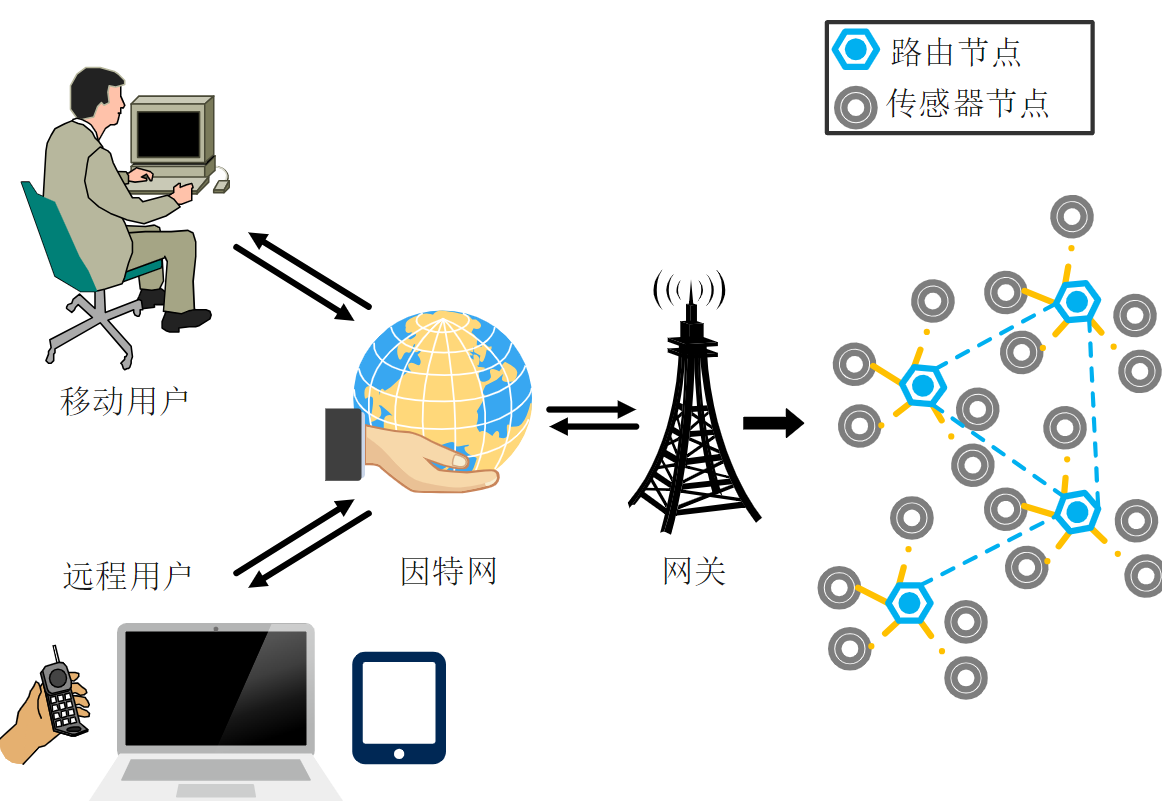
\includegraphics[width=0.75\textwidth]{1-1}
\caption{无线传感器网络体系结构}\label{Fig1-1}
\vspace*{10pt}
\end{figure}


\textcolor[rgb]{1.00,0.00,0.00}{1. 图要精选,具有自明性,切忌与表及文字表述重复。图要清楚,但坐标比例不要过分放大,同一图上不同曲线的点要分别用不同形状的标识符标出。地图插图涉及中国地图全图时,须使用自然资源部标准地图底图制作。}

\textcolor[rgb]{1.00,0.00,0.00}{2. 图序与图名置于图的下方,用宋体 5 号字,居中,段前空 6 磅,段后空 12 磅,单倍行距;图序与图名文字之间空一个字符。如“图 2-1 发展中国家经济增长速度的比较(1960-2000)”,其中“图 2-1”是图序。}

\textcolor[rgb]{1.00,0.00,0.00}{3. 图中的术语、符号、单位等应与正文表述中所用一致,图中文字用 5 号或小 5 号(9~10.5 磅)字,以能够清晰阅读为标准。专用名字代号、单位可采用外文表示,坐标轴题名、词组、描述性的词语均须采用中文。}

\textcolor[rgb]{1.00,0.00,0.00}{4. 如果一个图由两个或两个以上分图组成时,各分图分别以 (a)、(b)、(c)……作为图序,并须有分图名。}


\begin{figure}[htbp]
	\vspace*{6pt}
	\centering
	\subfigure[ ${\rho _1} + {\rho _2} = 3$ ]{\label{fig:subfig:1-2a}
		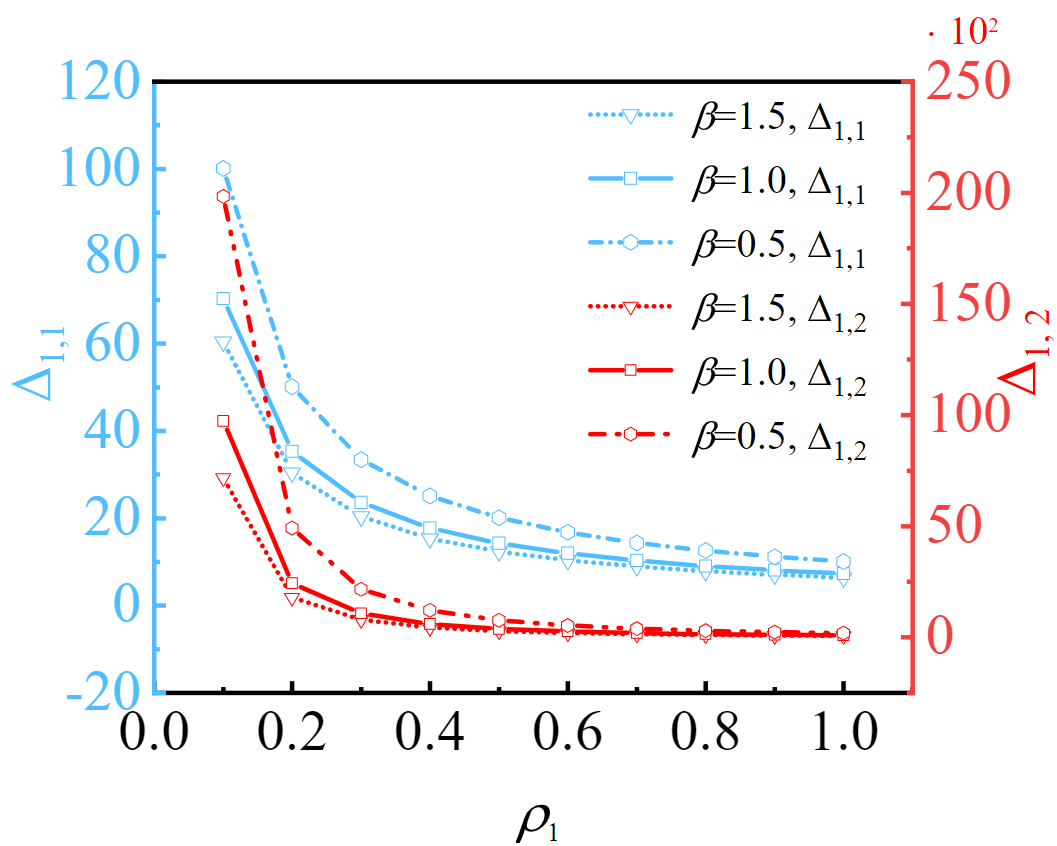
\includegraphics[width=0.48\textwidth]{1-2a}}
	\vspace{1pt}
	\subfigure[${\rho _1} + {\rho _2} = 4$]{\label{fig:subfig:1-2b}
		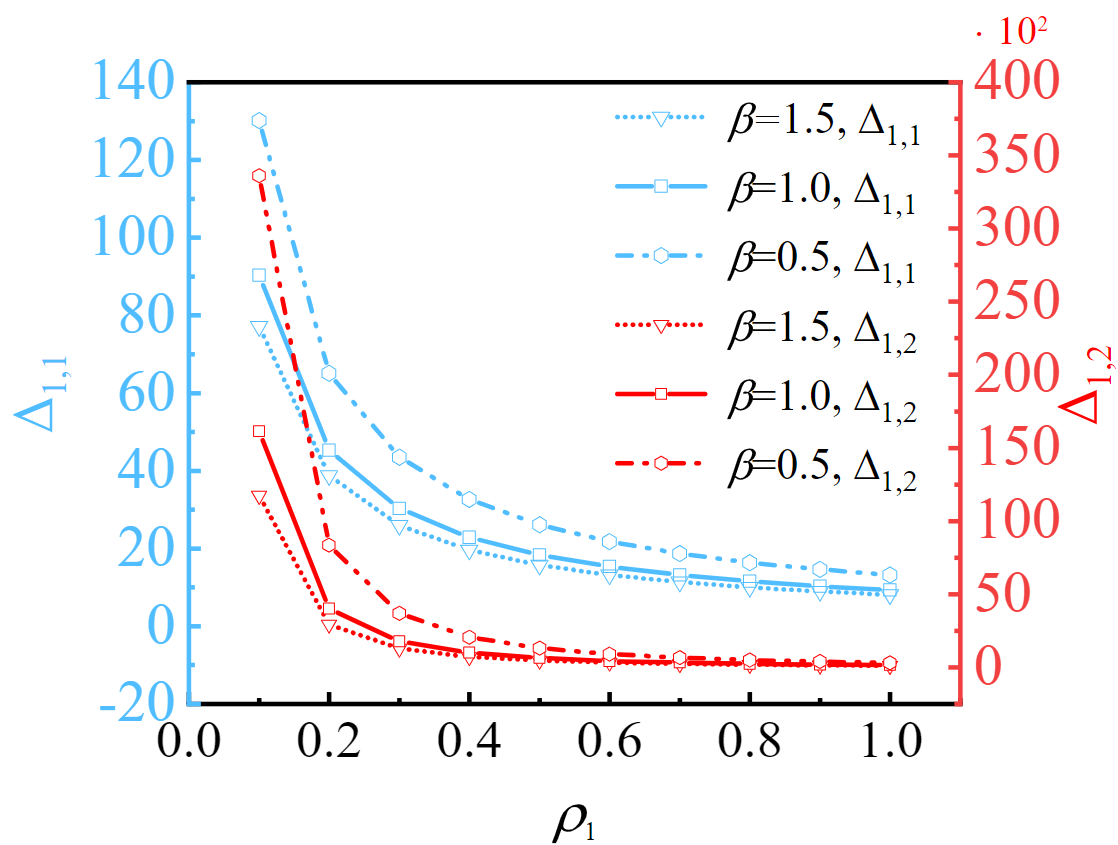
\includegraphics[width=0.48\textwidth]{1-2b}}
	\caption{$B = 1$,$\mu  = 1$设置下的平均 AoI${\Delta _{1,1}}$,方差 ${\Delta _{1,2}}$}\label{Fig1-2}
	\vspace*{10pt}
\end{figure}
图\ref{Fig1-2}给出$B = 1$设定下系统负载 $\rho$对 AoI 一阶矩,AoI 二阶矩的影响。分析图\ref{Fig1-2}可知,AoI 的一阶矩随 ${\rho_1}$的增大而逐渐降低。这时因为 ${\rho _1}$较小意味着系统中缺乏源${S_1}$新生成的状态更新包,这时服务器必须等待很长一段时间才能收到源${S_1}$的一个数据包,此时较长的等待时间会使得 AoI 的一阶矩较大。



\subsection{表的说明}

表\ref{Table1-1}显示了 5 个不同数据集的聚类准确率比较结果。该算法比较了在数据空间和用深度自动编码器编码后的特征空间的两种算法在数据的训练集和测试集上的聚类效果。从表中可以看出,不论任何数据集通过 SAE 编码后的聚类表现比直接进行聚类的表现更好,聚类准确率 ACC 有大幅度提高。这说明使用 SAE 提取数据的潜在特征,然后在数据集的特征空间进行聚类是有利的。这也说明了这些数据中存在着较多的冗余,经过了编码后的特征表现出更加清晰可分的结构。
\vspace{0.5em}
\begin{table}[ht!]
\centering
\caption { 不同聚类算法的聚类准确率比较 }\label{Table1-1}
\begin{tabular}{cccccc}
\hline \multirow{2}{*}{数据集 } & \multicolumn{2}{c}{SOM} & \multicolumn{2}{c}{提出的方法 } & \multirow{2}{*}{网络结构 } \\ \cline{2-5}
                 & 训练集        & 测试集        & 训练集         & 测试集  & \\
\hline  Iris     & 88.75 \% & 89.47 \% & 94.49 \% & 93.93 \% & \text { D-100-50-10-3 } \\
        Wine     & 91.52 \% & 90.59 \% & 96.24 \% & 95.56 \% & \text { D-100-50-10-3 } \\
        Isolet   & 58.82 \% & 57.68 \% & 66.42 \% & 64.7 \% & \text { D-500-100-30-26 } \\
        COIL-20  & 68.83 \% & 67.32 \% & 71.72 \% & 70.85 \% & \text { D-500-100-30-20 } \\
        MNIST    & 52.89 \% & 52.92 \% & 71.54 \% & 70.61 \% & \text { D-500-100-30-10 } \\
\hline
\end{tabular}
\end{table}

\textcolor[rgb]{1.00,0.00,0.00}{1. 表格一般应采用三线表(必要时可加辅助线),即表的上、下边线为单直线,线粗为 1.5 磅,第三条线为单直线,线粗为 1 磅。当三线表无法清晰表达时,可采用其他格式。}

\textcolor[rgb]{1.00,0.00,0.00}{2. 表中参数应标明量和单位的符号。表单元格中的文字一般用宋体 5 号或小 5 号字,居中(上下、左右均居中),单倍行距,段前空 3 磅,段后空 3 磅。不宜左右居中时,可采取两端对齐的方式。}

\textcolor[rgb]{1.00,0.00,0.00}{3. 表序与表名置于表的上方,用宋体 5 号字,居中,段前空 12 磅,段后空 6 磅,单倍行距,表序与表名文字之间空一个字符。如“表 3-1 XXX”,其中“表 3.1”是表序。}

\textcolor[rgb]{1.00,0.00,0.00}{4. 正文中表 1-1 前后没有空格。}

\textcolor[rgb]{1.00,0.00,0.00}{5. 表序、表名与表格应在同一页。当表格较大,不能在一页内打印时,可以“续表”形式另页打印,格式同前,只需在每页表序前加“续”字即可,例如“续表 3.1 XXX”。}

\textcolor[rgb]{1.00,0.00,0.00}{6. 表下方资料来源等文字说明,用宋体五号字,单倍行距,段前空 6 磅,段后空 12 磅。有续表时,资料来源注明在续表之下。}

\textcolor[rgb]{1.00,0.00,0.00}{7. 表格无特殊事由,一般不得截图。}

\subsection{公式的说明}

李雅普诺夫优化的本质是李雅普诺夫漂移,假设一个长度为$Ns$的系统队列,表示为向量组$Q\left( t \right) = \left( {{Q_1}\left( t \right),{Q_2}\left( t \right), \ldots ,{Q_{Ns}}\left( t \right)} \right)$。需要注意的是,这些队列包括实际队列和虚拟队列(它们与实际队列表现相同,但底层的物理含义与实际队列不同),此处所有队列变量都是非负的。为了度量$Q\left( t \right)$的总量,定义$Q\left( t \right)$的二次李雅普诺夫函数如下:
\begin{equation}\label{Eq1-1}
L\left( {Q\left( t \right)} \right) \buildrel \Delta \over = \frac{1}{2}\sum\limits_{n = 1}^{Ns} {{\theta _n}{Q_n}{{\left( t \right)}^2}},
\end{equation}
其中,${\theta _n},n = 1,2, \ldots ,Ns$是标记不同队列重要性的权重系数,${\theta _n}$必须为大于等于零的正值。通常当系统中所有队列的权重相同时,${\theta _n} = 1$。从上述可以得知,式\eqref{Eq1-1}中$L\left( {Q\left( t \right)} \right)$是非负的,当且仅当所有队列都为零时,它的值为零。

\textcolor[rgb]{1.00,0.00,0.00}{1. 表达式采用与正文相同的字号,单倍行距,居中或另起一段空两个汉字符书写(只能采用两种格式中的一种,全文须保持一致),段前空 6 磅,段后空 6 磅。}

\textcolor[rgb]{1.00,0.00,0.00}{2. 表达式的序号用括号,置于表达式右边行末,序号与表达式之间不加任何连线。}

\textcolor[rgb]{1.00,0.00,0.00}{3. 表达式在文字叙述中采用“式(3-1)”形式,在编号中用“(3-1)”形式。}

\textcolor[rgb]{1.00,0.00,0.00}{4. 公式中的字体为“Times New Roman”并斜体,大小可以在公式编辑器中自行设置,尽量让同一公式出现在同一行。}

\textcolor[rgb]{1.00,0.00,0.00}{5. 论文中出现的公式和参数字符一律用公式编辑器(如果没有用 mathtype)编写(不包括专有名词缩和其缩写),正文中公式出现显示不完整时,调整该行行间距为单倍行间距即可。}

\subsection{定理、推论、命题等的说明}

%定理
\begin{TheoremJXD}\label{Theorem1-1}
{考虑一个二次李雅普诺夫函数$L\left( {Q\left( t \right)} \right)$且$\mathbb{E}\left\{ {L\left( {Q\left( 0 \right)} \right)} \right\} < \infty $ ,假设此处的变量$B > 0$且$\varepsilon  \ge 0$,那么则有:
\begin{equation}\label{Eq1-2}
\Phi \left( {Q\left( t \right)} \right) \le B - \varepsilon \sum\limits_{n = 1}^{Ns} {\left| {{Q_n}\left( t \right)} \right|}.
\end{equation}
对所有的$Q\left( t \right)$都成立,从而有:
\begin{enumerate}
	\item {如果$\varepsilon  \ge 0$,则所有队列${Q_n}\left( t \right)$都是速率稳定的;}
	\item {如果$\varepsilon  > 0$,则所有队列都是强稳定的,并且有:
\begin{equation}\label{Eq1-3}
\mathop {\lim }\limits_{t \to \infty } \sup \frac{1}{t}\sum\limits_{\tau  = 0}^{t - 1} {\sum\limits_{n = 1}^{Ns}\mathbb{E} {\left\{ {\left| {{Q_n}\left( \tau  \right)} \right|} \right\}} }  \le \frac{B}{\varepsilon }.
\end{equation}	
}
\end{enumerate}
}
\end{TheoremJXD}
\vspace{0.5em}
上述\TheoremJXDref{Theorem1-1}给出了李雅普诺夫漂移界的队列稳定性条件。这个李雅普诺夫漂移的边界决定了系统中队列的稳定性。所有希望有效地保持稳定队列的算法都应该设计一种机制来实现这一界限。这一事实使得李雅普诺夫优化的框架易于识别。几乎所有利用李雅普诺夫优化的算法都可以分为两部分:第一部分努力满足上述定理的条件,从而使得队列稳定,而第二部分旨在实现一些系统目标,如吞吐量,功耗等,但这两部分并不是完全分开的,他们是由下面将要介绍的一些控制变量连接起来的。

%引理
\begin{LemmaJXD}\label{Lemma1-1}
考虑一个二次李雅普诺夫函数$L\left( {Q\left( t \right)} \right)$且$\mathbb{E}\left\{ {L\left( {Q\left( 0 \right)} \right)} \right\} < \infty $ ,假设此处的变量$B > 0$且$\varepsilon  \ge 0$,那么则有:
\begin{equation}\label{Eq1-4}
\Phi \left( {Q\left( t \right)} \right) \le B - \varepsilon \sum\limits_{n = 1}^{Ns} {\left| {{Q_n}\left( t \right)} \right|}.
\end{equation}
\end{LemmaJXD}
\vspace{0.5em}
上述\LemmaJXDref{Lemma1-1}给出了李雅普诺夫漂移界的队列稳定性条件。


%推论
\begin{CorollaryJXD}\label{Corollary1-1}
考虑一个二次李雅普诺夫函数$L\left( {Q\left( t \right)} \right)$且$\mathbb{E}\left\{ {L\left( {Q\left( 0 \right)} \right)} \right\} < \infty $ ,假设此处的变量$B > 0$且$\varepsilon  \ge 0$,那么则有:
\begin{equation}\label{Eq1-5}
\Phi \left( {Q\left( t \right)} \right) \le B - \varepsilon \sum\limits_{n = 1}^{Ns} {\left| {{Q_n}\left( t \right)} \right|}.
\end{equation}
\end{CorollaryJXD}
\vspace{0.5em}
上述\CorollaryJXDref{Corollary1-1}给出了李雅普诺夫漂移界的队列稳定性条件。


%定义
\begin{DefinitionJXD}\label{Definition1-1}
考虑一个二次李雅普诺夫函数$L\left( {Q\left( t \right)} \right)$且$\mathbb{E}\left\{ {L\left( {Q\left( 0 \right)} \right)} \right\} < \infty $ ,假设此处的变量$B > 0$且$\varepsilon  \ge 0$,那么则有:
\begin{equation}\label{Eq_2_3}
\Phi \left( {Q\left( t \right)} \right) \le B - \varepsilon \sum\limits_{n = 1}^{Ns} {\left| {{Q_n}\left( t \right)} \right|}.
\end{equation}
\end{DefinitionJXD}
\vspace{0.5em}
上述\DefinitionJXDref{Definition1-1}给出了李雅普诺夫漂移界的队列稳定性条件。


%命题
\begin{PropositionJXD}\label{Proposition1-1}
考虑一个二次李雅普诺夫函数$L\left( {Q\left( t \right)} \right)$且$\mathbb{E}\left\{ {L\left( {Q\left( 0 \right)} \right)} \right\} < \infty $ ,假设此处的变量$B > 0$且$\varepsilon  \ge 0$,那么则有:
\begin{equation}\label{Eq_2_3}
\Phi \left( {Q\left( t \right)} \right) \le B - \varepsilon \sum\limits_{n = 1}^{Ns} {\left| {{Q_n}\left( t \right)} \right|}.
\end{equation}
\end{PropositionJXD}
\vspace{0.5em}
上述\PropositionJXDref{Proposition1-1}给出了李雅普诺夫漂移界的队列稳定性条件。


\subsection{算法的描述}
在该算法中,提取特征阶段 SAE 采用逐层训练的方式对数据进行降维,在 mini-batch 模式下使用梯度下降进行优化,误差函数采用均方误差来减少损失。在训练过程中,SAE 首先通过第一层的编码器把原始数据编码特征,再通过解码函数把特征重构出输入数据,通过对原始数据和重构数据之间的误差进行比较,采用梯度下降对误差函数进行优化,更新本层编码器的参数,直到满足停止条件(误差足够小和到达最大迭代次数)后再依照第一层的训练过程进行下一层的训练任务。每层编码器都经过训练后训练完成。算法\ref{Algorithm1-1}详细描述了提取特征阶段的训练过程。在该算法中,提取特征阶段 SAE 采用逐层训练的方式对数据进行降维,在 mini-batch 模式下使用梯度下降进行优化,误差函数采用均方误差来减少损失。在训练过程中,SAE 首先通过第一层的编码器把原始数据编码特征,再通过解码函数把特征重构出输入数据,通过对原始数据和重构数据之间的误差进行比较,采用梯度下降对误差函数进行优化,更新本层编码器的参数,直到满足停止条件(误差足够小和到达最大迭代次数)后再依照第一层的训练过程进行下一层的训练任务。每层编码器都经过训练后训练完成。算法\ref{Algorithm1-1}详细描述了提取特征阶段的训练过程。
\vspace{10pt}
\begin{algorithm}[htb]	
	\setstretch{1.5}
 	\caption{训练堆叠自动编码器(提取特征阶段)}\label{Algorithm1-1}
	\begin{algorithmic}
		\wuhao
		\STATE \textbf{输入:}
        $\boldsymbol{X}=\left\{\boldsymbol{x}_1, \boldsymbol{x}_2, \cdots, \boldsymbol{x}_N\right\}$, batch 的大小 $b$, SAE 层数 $L$
        \STATE \textbf{输出:}	
         $\boldsymbol{H}=\left\{\boldsymbol{h}_1, \cdots, \boldsymbol{h}_N\right\}$ \\
        \vspace{0.3em}
        \hrule	
        \vspace{0.3em}		
        \STATE \textbf{1. }	
		初始化每层堆叠自动编码器的权值$\boldsymbol{W}_D^l$和偏差$\boldsymbol{b}_D^l$\\
        \STATE \textbf{2. }
        \textbf { for } $l \leftarrow 1$ \textbf { to } $L$ \textbf { do } \\
        \STATE \textbf{3. }
        \textbf { repeat} \\
        \STATE \textbf{4. }
        计算 $\boldsymbol{h}_i^{l-1}\left(\boldsymbol{h}_i^0=\boldsymbol{x}_i\right)$ 编码后的特征 $\boldsymbol{h}_i^l$ \\
        \STATE \textbf{5. }
        计算$\boldsymbol{h}_i^l$ 解码后产生的重构 $\tilde{\boldsymbol{h}}_i^{l-1}\left(\tilde{\boldsymbol{h}}_i^0=\tilde{\boldsymbol{x}}_i\right)$ \\
        \STATE \textbf{6. }
        计算$\boldsymbol{h}_i^l$和 $\tilde{\boldsymbol{h}}_i^{l-1}\left(\tilde{\boldsymbol{h}}_i^0=\tilde{\boldsymbol{x}}_i\right)$之间的误差  \\
        \STATE \textbf{7. }
        采用梯度下降优化更新参数$\theta^l=\left\{\boldsymbol{W}_D^l, \boldsymbol{b}_D^l\right\}$ \\
        \STATE \textbf{8. }
        \textbf {until} 满足停止条件 
        \STATE \textbf{9. }
        \textbf {end for}
	\end{algorithmic}
\end{algorithm}



\section{国内外研究现状}

参考文献的引用分为两种情况,一种是间接引用(上标)\cite{2004-David-Order},另一种是直接引用\mycite{2004-David-Order}。


主要包含以下几类参考文献:

1. 图书\mycite{2004-David-Order}

2. 期刊论文\mycite{2022-Jiao-TVT,2022-Guo-SP}

3. 会议论文\mycite{2015-Pappas-ICC}

4. 学位论文\mycite{2018-BUT}

其余请大家根据需要自行补充


\section{本文研究内容}

本文主要的研究内容如下:

(1)……

(2)

(3)


\section{论文结构安排}

本文从室内位置服务研究背景和无线定位算法研究现状出发,重点针对基于 Wi-Fi 的室内定位算法开展了深入的学习研究。论文结构安排如下:

第 1 章 绪论。首先介绍了基于位置服务中室内定位技术的研究背景和意义,然后简要概述了基于位置服务的体系结构、定位算法研究现状,最后阐述了本论文主要工作和结构安排。





\chapter{输入标题}

第 2 章,第 3 章,……,结论的写法这是论文作者的研究内容,不能将他人研究成果不加区分地掺和进来。已经在引言的文献综述部分讲过的内容,这里不需要再重复。

\section{一级标题}

具体内容 XXX

\subsection{二级标题}

具体内容 XXX

\subsection{二级标题}

具体内容 XXX

\section{一级标题}

具体内容 XXX

\subsection{二级标题}

具体内容 XXX

\subsection{二级标题}

具体内容 XXX

\section{一级标题}

具体内容 XXX

\subsection{二级标题}

具体内容 XXX

\subsection{二级标题}

具体内容 XXX

\section{本章小结}
具体内容 XXX



\chapter{输入标题}

具体内容 XXX

\section{一级标题}

具体内容 XXX

\subsection{二级标题}

具体内容 XXX

\subsection{二级标题}

具体内容 XXX

\section{一级标题}

具体内容 XXX

\subsection{二级标题}

具体内容 XXX

\subsection{二级标题}

具体内容 XXX

\section{一级标题}

具体内容 XXX

\subsection{二级标题}

具体内容 XXX

\subsection{二级标题}

具体内容 XXX

\section{本章小结}
具体内容 XXX



\chapter{输入标题}
具体内容 XXX

\section{一级标题}

具体内容 XXX

\subsection{二级标题}

具体内容 XXX

\subsection{二级标题}

具体内容 XXX

\section{一级标题}

具体内容 XXX

\subsection{二级标题}

具体内容 XXX

\subsection{二级标题}

具体内容 XXX

\section{一级标题}

具体内容 XXX

\subsection{二级标题}

具体内容 XXX

\subsection{二级标题}

具体内容 XXX

\section{本章小结}
具体内容 XXX

\chapter{输入标题}

具体内容 XXX

\section{一级标题}

具体内容 XXX

\subsection{二级标题}

具体内容 XXX

\subsection{二级标题}

具体内容 XXX

\section{一级标题}

具体内容 XXX

\subsection{二级标题}

具体内容 XXX

\subsection{二级标题}

具体内容 XXX

\section{一级标题}

具体内容 XXX

\subsection{二级标题}

具体内容 XXX

\subsection{二级标题}

具体内容 XXX

\section{本章小结}
具体内容 XXX



\addcontentsline{toc}{chapter}{结\quad 论}
\chapter*{结\quad 论}

学位论文的结论作为论文正文的最后一章单独排写,但不加章标题序号。
结论应是作者在学位论文研究过程中所取得的创新性成果的概要总结,不能与摘要混为一谈。学位论文结论应包括论文的主要结果和创新点、研究展望两部分,在结论中应概括论文的核心观点,明确、客观地指出本研究内容的创新性成果(含新见解、新观点、方法创新、技术创新、理论创新),并指出今后进一步在本研究方向进行研究工作的展望与设想。对所取得的创新性成果应注意从定性和定量两方面给出科学、准确的评价,分(1)、(2)、(3)…条列出,宜用“提出了”、“建立了”等词叙述。
结论是对论文主要研究结果、论点的提炼与概括,应准确、简明,完整,有条理,使人看后就能全面了解论文的意义、目的和工作内容。主要阐述自己的创造性工作及所取得的研究成果在本学术领域中的地位、作用和意义。同时,要严格区分自己取得的成果与导师及他人的科研工作成果。
在评价自己的研究工作成果时,要实事求是,除非有足够的证据表明自己的研究是“首次”的,“领先”的,“填补空白”的,否则应避免使用这些或类似词语。


%%%%%%%%%% 正文部分内容  %%%%%%%%%%


%%%%%%%%%%  参考文献  %%%%%%%%%%
\defaultfont
\bibliographystyle{NWNUThesis}
\phantomsection
\addcontentsline{toc}{chapter}{参考文献}            % 参考文献加入到中文目录
%\nocite{*}                                        % 若将此命令屏蔽掉,则未引用的文献不会出现在文后的参考文献中。
\bibliography{references}
\addcontentsline{toc}{chapter}{致\quad 谢} %添加到目录中
\chapter*{致\quad 谢}
\setlength{\parindent}{2em}
衷心感谢导师 XXX 教授对本人的精心指导。他的言传身教将使我终生受益。

感谢 XXX 教授,以及实验室全体老师和同窗们的热情帮助和支持!

本课题承蒙 XXXX 基金资助,特此致谢。


\addcontentsline{toc}{chapter}{附\quad 录} %添加到目录中
\chapter*{附\quad 录}
\setlength{\parindent}{2em}

\textcolor[rgb]{1.00,0.00,0.00}{(不需要的可不列此部分)}

附录是与论文内容密切相关、但编入正文又影响整篇论文编排的条理和逻辑性的一些资料,如某些重要的数据表格、计算程序、统计表等,是论文主体的补充内容,可根据需要设置。
附录的格式与正文相同,并依顺序用大写字母“A,B,C,……”或汉字“一,
二,三,……”编序号,如“附录 A,附录 B,附录 C,……”或“附录一,附录二,附录三,……”。只有一个附录时也要编序号,即附录 A。每个附录应有标题。附录序号与附录标题之间空一个字符,例如:“附录 A 甘肃省 2018 年度人口统计数据”。
附录中的图、表、数学表达式、参考文献等另行编序号,与正文分开,一律用阿拉伯数字编码,但在数码前冠以附录的序号,例如“图 A-1”,“表 B-2”,“式(C-3)”等。

\addcontentsline{toc}{chapter}{个人简历、在学期间研究成果及科研项目}
\chapter*{个人简历、在学期间发表的学术论文及研究成果}
\setlength{\parindent}{0pt}
\qquad {\heiti{\sihao1. 个人简历}}
\vspace*{0.3em}
\begin{publist}
	\item XXXX 年 XX 月 XX 日出生于 XXXX。
	\item XXXX 年 XX 月——XXXX 年 XX 月,在 XX 大学 XX 学院(系)XX 专业本科毕业并获得 XX 学学士学位。
	\item XXXX 年 XX 月——至今,在 XX 大学 XX 学院(系)XX 学科攻读 XX 学硕士学位。
\end{publist}
%注:个人简历包括出生年月日、获得学士、硕士学位的学校、时间等,格式同正文论文段落格式。

\qquad {\heiti{\sihao2. 在学期间发表的学术论文}}
\vspace*{0.3em}
\begin{publist}
	\item XXX, XXX. Static Oxidation Model of Al-Mg/C Dissipation Thermal Protection Materials[J]. Rare Metal Materials and Engineering, 2010, 39(1):520–524. (SCI 收录)
	\item XXX, XXX. 精密超声振动切削单晶铜的计算机仿真研究 [J]. 系统仿真学报,2007, 19(4):738–741, 753.
	\item XXX, XXX. 局部多孔质气体静压轴向轴承静态特性的数值求解 [J]. 摩擦学学报,2007(1):68–72.
    \item XXX, XXX. 硬脆光学晶体材料超精密切削理论研究综述 [J]. 机械工程学报,2003, 39(8):15–22.
\end{publist}
\vspace*{1em}
\qquad {\heiti{\sihao3. 在学期间申请的软件著作权及专利}}
\vspace*{0.3em}
\begin{publist}
   \item XXX, XXX. 基于大数据的智慧商城微信小程序软件 V1.0. 登记号:XXXX(软件著作权,已登记)
   \item XXX, XXX. 一种基于物联网的温控机构。申请号:XXXXXX(实用新型,已授权)
\end{publist}
\vspace*{1em}
\qquad {\heiti{\sihao4. 在学期间主持和参与的科研项目}}
\vspace*{0.3em}
\begin{publist}
	\item	2022 年度甘肃省教育厅优秀研究生“创新之星”项目:基于信息新鲜度的多接入传感网络调度策略研究,项目编号:XXXX。(主持)
	\item	国家自然科学基金项目:面向 B5G 的毫米波大规模 MIMO 低空无人机异构网络信道模型及其回程应用,项目编号:XXXX, 执行期限:2019/01-2022/12。(参与)
\end{publist}
%\vfill
\hangafter=1\hangindent=2em\noindent
                   % 发表论文和参加科研情况说明              % 致谢
\clearpage
\end{CJK*}                                        % 结束中文字体使用
\end{sloppypar}
\end{document}                                    % 结束全文
